\chapter{Numerical Experiments}\label{chap: experiments}

In the previous sections, we derived general framework for classification at the top and showed that multiple well-known formulations fall into it. The summary of all formulations presented in this work is in Table~\ref{tab: summary formulations}. The goal of this chapter is to experimentally verify the properties of these formulations. 

\section{Settings}\label{sec: settings}

In this section we describe in detail all settings used for experiments. 

\subsection{Formulations}

Formulations from Table~\ref{tab: summary formulations} can be divided into three categories:
\begin{itemize}
  \item The first category contains \TopPush and \TopPushK formulations. Formulations from this category minimize the surrogate approximation of the false-negative rate. As a threshold, these formulations use the mean of a small fraction of the negative samples with the highest scores.
  \item The second category consists of \Grill, \TopMeanK, and \PatMat formulation. These three formulations again use the surrogate approximation of the false-negative rate as an objective function. The only exception is the \Grill formulation also adds the surrogate approximation of the false-positive rate into the objective function for better stability. All three formulation uses some kind of approximation of the top $\tau$-quantile of all scores as a threshold.
  \item The last category consists of \GrillNP, \tauFPL, and \PatMatNP. These formulations use the same objectives as their corresponding formulations from the previous category and differ only in the definition of the decision threshold. All three formulation uses some kind of approximation of the top $\tau$-quantile of negative scores as a threshold.
\end{itemize}
To simplify the setup of all experiments, we decided to focus on formulations that use only negative samples for the threshold computation, i.e. formulations from the first and third categories. The performance of these formulations can be easily compared using some basic performance metrics as we show later in Section~\ref{sec: performance criteria}.

In total, we use four different formulations from Table~\ref{tab: summary formulations}, namely \TopPush, \TopPushK, \tauFPL, and \PatMatNP. We decided to omit the \GrillNP formulation in final experiments, because it provides very poor results in preliminary experiments. Moreover, for \TopPushK we use two different values of~$K = \{5, 10\}$ and consider the resulting formulations as separate formulations, i.e. we have \TopPushK(5) and \TopPushK(10). Similarly, for \tauFPL and \PatMat we use two different values of~$\tau = \{0.01, 0.05\}.$ For all formulations, we use the hinge loss defined in Notation~\ref{not: surrogates} as a surrogate function.

We have a total of 7 different formulations, however, all these formulations fall into our general framework. To show that these formulations work properly, we have to compare them to some standard methods. In previous chapters, we showed how to solve presented formulations in their primal (Chapters~\ref{chap: linear} and~\ref{chap: deep}) and dual form (Chapter~\ref{chap: dual}). Whenever we use the primal form in the experiments, we use binary cross-entropy defined in the following way as a baseline formulation 
\begin{mini}{\bm{w}}{
  \frac{1}{\nall} \sum_{i \in \I} \Brac{- y_i \log(s_i) - (1 - y_i) \log (1 - s_i)}
  }{\label{eq: crossentropy}}{}
  \addConstraint{s_i}{= f(\bm{x}_i; \bm{w}), \quad i \in \I.}
\end{mini}
We decided to use binary cross-entropy, since it is one of the most used objective functions for binary classification in machine learning applications. In the following text, we will denote binary cross-entropy as \BaseLine for simplicity. In experiments with dual forms, we use C-SVC variant of SVM~\cite{boser1992training, cortes1995support,chang2011libsvm} defined as follows
\begin{mini}{\bm{w}, b, \bm{\xi}}{
  \frac{1}{2} \norm{\bm{w}}^2 + C \sum_{i \in \I} \xi_i
  }{\label{eq: SVM}}{}
  \addConstraint{y_i}{\Brac{\bm{w}^{\top} \phi(\bm{x}_i) + b} \geq 1 - \xi_i, \quad i \in \I}
  \addConstraint{\xi_i}{\geq 0, \quad i \in \I,}
\end{mini}
where~$y_i \in \{-1, 1\}$ for all~$i \in \I$ and~$\phi(\bm{x}_i)$ maps~$\bm{x}_i$ into a higher-dimensional space (see Section~\ref{sec: kernels}). The corresponding dual form is as follows
\begin{maxi}{\bm{\alpha}}{
  - \frac{1}{2} \bm{\alpha}^{\top} \K \bm{\alpha} - \sum_{i = 1}^{\nall} \alpha_i
  }{\label{eq: SVM dual}}{}
  \addConstraint{\sum_{i = 1}^{\nall} y_i \alpha_i}{= 0}
  \addConstraint{0 \leq \alpha_i }{\leq C, \quad i = 1, 2, \ldots, \nall,}
\end{maxi}
where the kernel matrix~$\K$ is defined as
\begin{equation*}
  \K_{i,j} = y_i y_j k(\bm{x}_i, \bm{x}_j) = \phi(\bm{x}_i)^{\top} \phi(\bm{x}_j),
\end{equation*}
for all~$i, j = 1, 2, \ldots, \nall.$ Note that the dual form of C-SVC is very similar to the dual forms of our formulations derived in Chapter~\ref{chap: dual}. In the following text, we will denote C-SVC as \SVM for simplicity.

In total, we have 9 different formulations. However, not all formulations are used for all experiments: \BaseLine formulation is also not used for experiments with dual forms, and \SVM is used only for experiments with dual forms. The summary of all formulations used for experiments is in Table~\ref{tab: formulations experiments summary}.

\subsection{Hyperparameters}

Since considered formulations differ in the number of available hyper-parameters, we decided to fix the number of hyper-parameters per formulation to six. For most of the considered formulations, the remaining hyper-parameter is the regularization constant~$\lambda$. The only exceptions are the formulations derived from \PatMatNP, since they also have the scaling parameter~$\vartheta.$ Therefore, we use the following six values of this hyper-parameter
\begin{equation*}
  \lambda \in \Brac[c]{10^{-5}, 10^{-4}, 10^{-3}, 10^{-2}, 10^{-1}, 1}
\end{equation*}
for all formulations except \PatMatNP. Since we used a slightly different (but equivalent) primal formulation for the derivation of the dual forms, we use~$\lambda$ to compute hyper-parameter~$C$ used in dual forms
\begin{equation*}
  C = \frac{1}{\lambda \ntil},
\end{equation*}
where~$\ntil = \nall$ for \SVM and~$\ntil = \npos$ otherwise. For formulations derived from \PatMatNP, we fixed~$\lambda$ to~$10^{-3}$ and use the following six different values of the scaling parameter
\begin{equation*}
  \vartheta \in \Brac[c]{10^{-5}, 10^{-4}, 10^{-3}, 10^{-2}, 10^{-1}, 1}.
\end{equation*}
In all experiments, the best hyperparameter is selected based on the validation data and the appropriate performance metric.

\begin{table}[!ht]
  \centering
  \begin{NiceTabular}{lcccc}
    \CodeBefore
      \rowcolor{\headercol}{1}
      \rowcolors{3}{\rowcol}{}[restart]
    \Body
    \toprule
    \textbf{Formulation}
      & \textbf{Fixed parameters}
      & \textbf{Hyper-parameter}
      & \textbf{Primal Form}
      & \textbf{Dual Form} \\
    \midrule
    \BaseLine
      & ---
      & $\lambda$
      & \yesmark
      & \nomark \\
    \SVM
      & ---
      & $\lambda$
      & \nomark 
      & \yesmark \\
    \midrule
    \TopPush
      & ---
      & $\lambda$
      & \yesmark
      & \yesmark \\
    \TopPushK(5)
      & $K = 5$
      & $\lambda$
      & \yesmark
      & \yesmark \\
    \TopPushK(10)
      & $K = 10$
      & $\lambda$
      & \yesmark
      & \yesmark \\
    \tauFPL(0.01)
      & $\tau = 0.01$
      & $\lambda$
      & \yesmark
      & \yesmark \\
    \tauFPL(0.05)
      & $\tau = 0.05$
      & $\lambda$
      & \yesmark
      & \yesmark \\
    \PatMatNP(0.01)
      & $\tau = 0.01,$ $\lambda = 0.001$
      & $\vartheta$
      & \yesmark
      & \yesmark \\
    \PatMatNP(0.05)
      & $\tau = 0.05,$ $\lambda = 0.001$
      & $\vartheta$
      & \yesmark
      & \yesmark \\
    \bottomrule
  \end{NiceTabular}
  \caption{Summary of all formulations used for experiments. The first column shows the aliases used for the formulations when describing the experiment results. The second column shows fixed hyperparameters used for each formulation, while the third column shows which hyper-parameters are tuned using validation data. The last two columns indicate whether the formulation is used in primal experiments, dual experiments, or both.}
  \label{tab: formulations experiments summary}
\end{table}

\subsection{Datasets}

For the numerical experiments, we consider variety of different datasets summarized in Table~\ref{tab: datasets summary}, that can be divided into three categories:
\begin{enumerate}
  \item \textbf{Image Recognition:} In this category, we test formulations from Table~\ref{tab: formulations experiments summary} on datasets from the domain of image recognition. We use this domain since it is one of the most popular domains these days, and therefore, there are plenty of publicly available datasets.
  \item \textbf{Steganalysis:} In this category, we use presented formulations in the domain of steganalysis. In this domain, the problem of maximizing the true-positive rate at the specific level of the false-positive rate is well-known as we show at the beginning of Section~\ref{sec: steganalysis}. Therefore, formulations from Table~\ref{tab: formulations experiments summary} can be very useful in this domain.
  \item \textbf{Malware Detection:} In this category, we use formulations for malware detection. Similar to steganalysis,  the problem of maximizing the true-positive rate at the specific level of the false-positive rate is crucial for malware detection as discussed at the beginning of Section~\ref{sec: malware detection}. Therefore, formulations from Table~\ref{tab: formulations experiments summary} can be very useful in this domain.
\end{enumerate}
For each of these categories, there is a separate section with results and a more detailed description later in the text. It is worth mentioning, that not all datasets that are used in experiments are primarily designed for the classification at the top. In fact, all datasets from the first category are general image classification datasets. We use these datasets for two reasons. The first one is that they are publicly available. The second reason is, that all these datasets are well-known, and therefore it is easier to present the results on them.

\begin{table}[!ht]
  \centering
  \resizebox{\columnwidth}{!}{%
    \begin{NiceTabular}{lccrrrrrr}
      \CodeBefore
      \rowcolor{\headercol}{1-2}
      \rowcolors{4}{\rowcol}{}[restart]
      \Body
      \toprule
      \Block[c]{2-1}{\textbf{Dataset}}
      & \Block[c]{2-1}{$y^+$}
      & \Block[c]{2-1}{$d$}
      & \Block[c]{1-2}{\textbf{Train}}
      && \Block[c]{1-2}{\textbf{Validation}}
      && \Block[c]{1-2}{\textbf{Test}} \\
      \cline{4-9}
      &&& \Block[c]{1-1}{$n$}
      & \Block[c]{1-1}{$\frac{\npos}{n}$}
      & \Block[c]{1-1}{$n$}
      & \Block[c]{1-1}{$\frac{\npos}{n}$}
      & \Block[c]{1-1}{$n$}
      & \Block[c]{1-1}{$\frac{\npos}{n}$} \\
      \midrule
      MNIST
      & 1
      & $28 \times 28 \times 1$
      & 45 000
      & 11.3\%
      & 15 000
      & 11.2\%
      & 10 000
      & 11.4\% \\
      FashionMNIST
      & 1
      & $28 \times 28\times 1$
      & 45 000
      & 10.0\%
      & 15 000
      & 9.9\%
      & 10 000
      & 10.0\% \\
      CIFAR10
      & 1
      & $32 \times 32 \times 3$
      & 37 500
      & 10.0\%
      & 12 500
      & 9.9\%
      & 10 000
      & 10.0\% \\
      CIFAR20
      & 1
      & $32 \times 32 \times 3$
      & 37 500
      & 5.0\%
      & 12 500
      & 5.1\%
      & 10 000
      & 5.0\% \\
      CIFAR100
      & 1
      & $32 \times 32 \times 3$
      & 37 500
      & 1.0\%
      & 12 500
      & 1.0\%
      & 10 000
      & 1.0\% \\
      SVHN2
      & 1
      & $32 \times 32\times 3$
      & 54 944
      & 18.9\%
      & 18 313
      & 18.9\%
      & 26 032
      & 19.6\% \\
      SVHN2-Extra
      & 1
      & $32 \times 32\times 3$
      & 453 291
      & 17.3\%
      & 151 097
      & 17.1\%
      & 26 032
      & 19.6\% \\
      \midrule
      \bad{Nsf5}
      & ---
      & $22 510 \times 1$
      & 186 583
      & 9.1\%
      & 62 194
      & 9.1\%
      & 248 776
      & 9.1\% \\
      \bad{JMiPOD}
      & ---
      & $256 \times 256\times 3$
      & 186 515
      & 9.1\%
      & 62 172
      & 9.1\%
      & 248 686
      & 9.1\% \\
      \midrule
      \bad{Malware}
      & ---
      & variable
      & 6 580 166
      & 87.22\%
      & ---
      & ---
      & 800 346
      & 91.8\% \\
      \bottomrule
    \end{NiceTabular}
  }
  \caption{Structure of the used datasets: The training, validation and testing sets show the positive label~$y^+,$ the number of features~$d$, samples~$n$ and the fraction of positive samples~$\frac{\npos}{n}$. Datasets depicted in red are not publicly available.}
  \label{tab: datasets summary}
\end{table}

\subsection{Performance Criteria}\label{sec: performance criteria}

In the previous subsections, we described all formulations and datasets used for the experiments. In this section, we describe which performance criteria are used for evaluation and how these criteria are related to the tested formulations.

As we discussed at the beginning of Section~\ref{sec: settings}, we decided to test only formulations that minimize the false-negative rate (or a combination of false-negative and false-positive rate) and use only negative samples for the threshold computation. This choice allows us to use simple metrics to compare used formulations. The first metric that we use in experiments is~$\tpratk$ defined as follows
\begin{equation*}
  \tpratk = \frac{1}{\npos} \sum_{i \in \Ipos} \Iverson{s_i \geq t} \quad \text{where} \quad t = \sum_{j = 1}^{K} s^{-}_{[j]}.
\end{equation*}
This metric computes the true-positive rate at threshold~$t$ which is the mean of $K$-largest negative scores. For~$K = 1$ the threshold corresponds to the threshold used by \TopPush formulation, and otherwise threshold~$t$ corresponds to the threshold used by \TopPushK. Moreover, since minimizing the false-negative rate is equivalent to maximizing the true-positive rate, both \TopPush and \TopPushK should optimize the $\tpratk$ metric. In the upcoming experiments, we use this metric with three different values of~$K \in \{1, 5, 10\}.$

The second metric is defined in a similar way
\begin{equation*}
  \tpratfpr = \frac{1}{\npos} \sum_{i \in \Ipos} \Iverson{s_i \geq t} \quad \text{where} \quad t
  = \max \Set{t}{\frac{1}{\nneg} \sum_{i \in \Ineg} \Iverson{s_i \geq t} \geq \tau}.
\end{equation*}
This metric computes the true-positive rate at a specific top $\tau$-quantile of negative scores. This metric is ideal for testing the performance of \tauFPL and \PatMatNP, since both formulations maximize true-positive rate and use some kind of approximation of the true top $\tau$-quantile of negative scores as a threshold. In experiments, we use this metric with two different values of~$\tau \in \{0.01, 0.05\}.$ 

The two previous metric are specific for the formulations from our framework. However, we should also test if the baseline formulations work properly. Since the baseline methods are designed to optimize overall perfomance, we use area under ROC curve to measure the overall performance. The summary of all used metrics is in Table~\ref{tab: metrics summary}.

\begin{table}[!ht]
  \centering
  \begin{NiceTabular}{lcccccc}
    \CodeBefore
    \rowcolor{\headercol}{1-2}
    \rowcolors{4}{\rowcol}{}[restart]
    \Body
    \toprule
    \Block[c]{2-1}{\textbf{Formulation}}
      & \Block[c]{2-1}{$\auroc$}
      & \Block[c]{1-3}{$\tpratk$}
      &&& \Block[c]{1-2}{$\tpratfpr$} \\
    \cline{3-7}
      && $1$  
      & $5$
      & $10$
      & $0.01$
      & $0.05$ \\
    \midrule
    \BaseLine
      & \yesmark
      & \nomark
      & \nomark
      & \nomark
      & \nomark
      & \nomark \\
    \SVM
      & \yesmark
      & \nomark
      & \nomark
      & \nomark
      & \nomark
      & \nomark \\
    \midrule
    \TopPush
      & \nomark
      & \yesmark
      & \nomark
      & \nomark
      & \nomark
      & \nomark \\
    \TopPushK(5)
      & \nomark
      & \nomark
      & \yesmark
      & \nomark
      & \nomark
      & \nomark \\
    \TopPushK(10)
      & \nomark
      & \nomark
      & \nomark
      & \yesmark
      & \nomark
      & \nomark \\
    \tauFPL(0.01) and \PatMatNP(0.01)
      & \nomark
      & \nomark
      & \nomark
      & \nomark
      & \yesmark
      & \nomark \\
    \tauFPL(0.05) and \PatMatNP(0.05)
      & \nomark
      & \nomark
      & \nomark
      & \nomark
      & \nomark
      & \yesmark \\
    \bottomrule
  \end{NiceTabular}
  \caption{The summary of all used perofmance metrics used for evaluation. In total we use six different metrics and eleven different formulations. For each formulation~\yesmark denotes the metric in which the formulation should be the best.}
  \label{tab: metrics summary}
\end{table}

\subsection{Critical Difference Diagrams}\label{sec: cd evaluation}

All metrics from Section~\ref{sec: performance criteria} can be used to compare different formulations on a single dataset. However, these metrics are not suitable for comparison of multiple formulations on multiple datasets. To address this issue, we follow the suggestion from~\cite{demvsar2006statistical} and use the Friedman test~\cite{friedman1940comparison}. Consider that we have~$D,$ datasets and~$k$ formulations. Than for each dataset~$i$, each formulation~$j$ is ranked by rank~$r^i_j$ according to some performance criterium (any performance metric from previous section), i.e. the formulation that provides the best result has rank 1, the second best has rank 2, etc.. If two formulations provides the same results, the average ranks are assigned. The average rank over all dataset for formulation~$j$ is then computed as~$R_j = \frac{1}{D} \sum_{i = 1}^{D} r^{i}_{j}.$ The Friedman test compares the average ranks of formulations under the null hypothesis, which states that all formulations are equivalent and therefore their average ranks should be equal. If the null hypothesis is rejected, we proceed with the post-hoc Nemenyi test~\cite{nemenyi1963distribution} that compares all formulations to each other. The performance of two formulations is significantly different if the corresponding average
ranks differ by at least the critical difference
\begin{equation*}
  CD = q_{\alpha} \sqrt{\frac{k(k + 1)}{6D}},
\end{equation*}
where critical values~$q_{\alpha}$ are based on the Studentized range statistic divided by~$\sqrt{2},$ see Table 5(a) in~\cite{demvsar2006statistical}. The results of this post hoc test can be easily visualized using critical difference diagrams proposed in~\cite{demvsar2006statistical}.  The $x$-axis of such diagram shows the average rank over all datasets for each formulation. Formulations that are not significatnly different according to the Nemenyi test are connected using green horizontal line. As an example of such diagrams see Figure~\ref{fig: critical diagrams primal}.

\subsection{Implementation}

For the implementation of all formulations we use the Julia programming language~\cite{bezanson2017julia}. The dual formulations are implemented from scratch in pure Julia, while the primal formulations are implemented using Flux.jl~\cite{innes:2018, Flux.jl-2018} library. This library provides all the necessary tools for building neural networks. Moreover, the library allows the implementation of a custom gradient for any function, which allows us to implement all formulations from Table~\ref{tab: summary formulations}. For experiments with SVM, we use the Julia wrapper for the LIBSVM library~\cite{chang2011libsvm}. All codes used for experiments as well as all configurations of all experiments are publicly available on GitHub:
\begin{center}
  \url{https://github.com/VaclavMacha/ClassificationAtTopExperiments.jl}
\end{center}

\section{Image Recognition}

This section contains results for six well-known visual recognition datasets. MNIST \cite{deng2012mnist} and FashionMNIST \cite{xiao2017fashionmnist} are grayscale datasets of digits and fashion items, respectively. CIFAR100~\cite{krizhevsky2009learning} is a dataset of coloured images of different items grouped into 100 classes. CIFAR10 and CIFAR20 merge these classes into 10 and 20 superclasses, respectively. Finally, SVHN2~\cite{netzer2011reading} contains coloured images of house numbers. All these datasets are originally divided only into training and test sets. Therefore, we select 25\% samples from the training set to obtain the validation set. For a more detailed description of the structure of datasets, see Table~\ref{tab: datasets summary}.


\subsection{Primal Formulation: Linear Model}\label{sec: results primal linear}

\begin{table}[!p]
  \centering
  \underline{$\tpratk =10$}
  \vspace{0.25cm}\\
  \resizebox{\columnwidth}{!}{% 
    \begin{NiceTabular}{lccccccc}
      \CodeBefore
        \rowcolor{\headercol}{1}
        \rowcolors{3}{\rowcol}{}[restart]
      \Body
      \toprule
      \textbf{Formulation}
        & \textbf{MNIST}
        & \textbf{FashionMNIST}
        & \textbf{CIFAR10}
        & \textbf{CIFAR20}
        & \textbf{CIFAR100}
        & \textbf{SVHN2}
        & \textbf{SVHN2Extra}\\
      \midrule
      \BaseLine
        & 68.54
        & 85.65
        & \worst{1.25}
        & \best{1.40}
        & \worst{2.00}
        & 0.04
        & \worst{0.02}\\
      \TopPush
        & 89.38
        & \best{93.70}
        & 2.25
        & \worst{0.40}
        & 4.00
        & \worst{0.02}
        & \worst{0.02}\\
      \TopPushK(5)
        & 89.60
        & 93.30
        & 3.30
        & 1.10
        & 3.00
        & 0.04
        & 0.06\\
      \TopPushK(10)
        & \best{89.64}
        & 92.75
        & 3.90
        & 0.70
        & 4.50
        & 0.04
        & \best{0.09}\\
      \tauFPL(0.01)
        & 83.35
        & 92.40
        & 2.90
        & 0.80
        & 2.50
        & 0.03
        & \worst{0.02}\\
      \tauFPL(0.05)
        & \worst{40.26}
        & \worst{79.65}
        & 3.60
        & 1.00
        & \best{5.50}
        & 0.04
        & \best{0.09}\\
      \PatMatNP(0.01)
        & 87.88
        & 92.75
        & \best{5.00}
        & 1.10
        & 4.00
        & 0.12
        & \best{0.09}\\
      \PatMatNP(0.05)
        & 51.72
        & 81.60
        & 3.80
        & 1.20
        & 3.00
        & \best{0.14}
        & 0.06\\
      \bottomrule
    \end{NiceTabular}
  }
  \vspace{0.25cm}\\
  \underline{$\tpratfpr = 0.05$}
  \vspace{0.25cm}\\
  \resizebox{\columnwidth}{!}{% 
    \begin{NiceTabular}{lccccccc}
      \CodeBefore
        \rowcolor{\headercol}{1}
        \rowcolors{3}{\rowcol}{}[restart]
      \Body
      \toprule
      \textbf{Formulation}
        & \textbf{MNIST}
        & \textbf{FashionMNIST}
        & \textbf{CIFAR10}
        & \textbf{CIFAR20}
        & \textbf{CIFAR100}
        & \textbf{SVHN2}
        & \textbf{SVHN2Extra}\\
      \midrule
      \BaseLine
        & \best{99.65}
        & 99.30
        & 43.40
        & 32.90
        & 54.50
        & 5.53
        & \worst{5.91}\\
      \TopPush
        & \worst{99.12}
        & \worst{98.30}
        & \worst{31.10}
        & \worst{16.30}
        & 43.50
        & \worst{5.22}
        & 6.40\\
      \TopPushK(5)
        & 99.21
        & \worst{98.30}
        & 35.50
        & 20.20
        & \worst{42.50}
        & 6.78
        & 7.42\\
      \TopPushK(10)
        & 99.30
        & \worst{98.30}
        & 37.90
        & 20.80
        & 46.50
        & 6.15
        & 8.07\\
      \tauFPL(0.01)
        & 99.47
        & 98.75
        & 35.85
        & 24.00
        & 44.00
        & 6.90
        & 7.76\\
      \tauFPL(0.05)
        & 99.56
        & 99.20
        & 39.50
        & 25.70
        & 50.50
        & 8.16
        & 9.69\\
      \PatMatNP(0.01)
        & 99.52
        & 98.85
        & 45.35
        & 33.70
        & 56.00
        & 9.28
        & \best{12.47}\\
      \PatMatNP(0.05)
        & \best{99.65}
        & \best{99.40}
        & \best{46.80}
        & \best{34.80}
        & \best{58.50}
        & \best{9.34}
        & 12.25\\
      \bottomrule
    \end{NiceTabular}
  }
  \vspace{0.25cm}\\
  \underline{$\auroc$}
  \vspace{0.25cm}\\
  \centering
  \resizebox{\columnwidth}{!}{% 
    \begin{NiceTabular}{lccccccc}
      \CodeBefore
        \rowcolor{\headercol}{1}
        \rowcolors{3}{\rowcol}{}[restart]
      \Body
      \toprule
      \textbf{Formulation}
        & \textbf{MNIST}
        & \textbf{FashionMNIST}
        & \textbf{CIFAR10}
        & \textbf{CIFAR20}
        & \textbf{CIFAR100}
        & \textbf{SVHN2}
        & \textbf{SVHN2Extra}\\
      \midrule
      \BaseLine
        & \best{99.86}
        & \best{99.83}
        & \best{84.00}
        & \best{76.26}
        & \best{88.48}
        & \best{57.82}
        & \best{56.10}\\
      \TopPush
        & \worst{99.78}
        & \worst{99.42}
        & \worst{73.84}
        & 65.76
        & 82.10
        & 51.08
        & 51.30 \\
      \TopPushK(5)
        & 99.8
        & \worst{99.42}
        & 76.67
        & \worst{65.70}
        & \worst{81.52}
        & \worst{50.98}
        & 50.69\\
      \TopPushK(10)
        & 99.82
        & 99.48
        & 77.74
        & 66.87
        & 81.91
        & 51.90
        & \worst{50.58}\\
      \tauFPL(0.01)
        & 99.84
        & 99.72
        & 77.34
        & 69.24
        & 82.96
        & 51.04
        & 50.62\\
      \tauFPL(0.05)
        & 99.81
        & 99.80
        & 79.41
        & 70.86
        & 84.56
        & 51.78
        & 50.76\\
      \PatMatNP(0.01)
        & 99.85
        & 99.68
        & 82.34
        & 74.56
        & 86.13
        & 56.38
        & 51.93\\
      \PatMatNP(0.05)
        & 99.84
        & 99.81
        & 83.35
        & 75.44
        & 87.22
        & 56.40
        & 52.50\\
      \bottomrule
    \end{NiceTabular}
  }
  \caption{\textbf{Primal formulation with linear model:} Each table corresponds to one performance metric and all presented results are medians of ten independent runs for each pair of datasets and formulation. The best result for each dataset is highlighted in green, while the worst result is highlighted in red.}
  \label{tab: primal auc}
\end{table}

One of the basic assumption of the critical difference diagrams to work properly is the large number of datasets. Since we perform all experiments for each formulation and each dataset ten times with different randomseed for train/valid/test split, we decided to consider each of this run as a separate dataset. It is important, that we use this settings only for the critical difference diagrams.

\begin{figure}[!p]
  \centering
  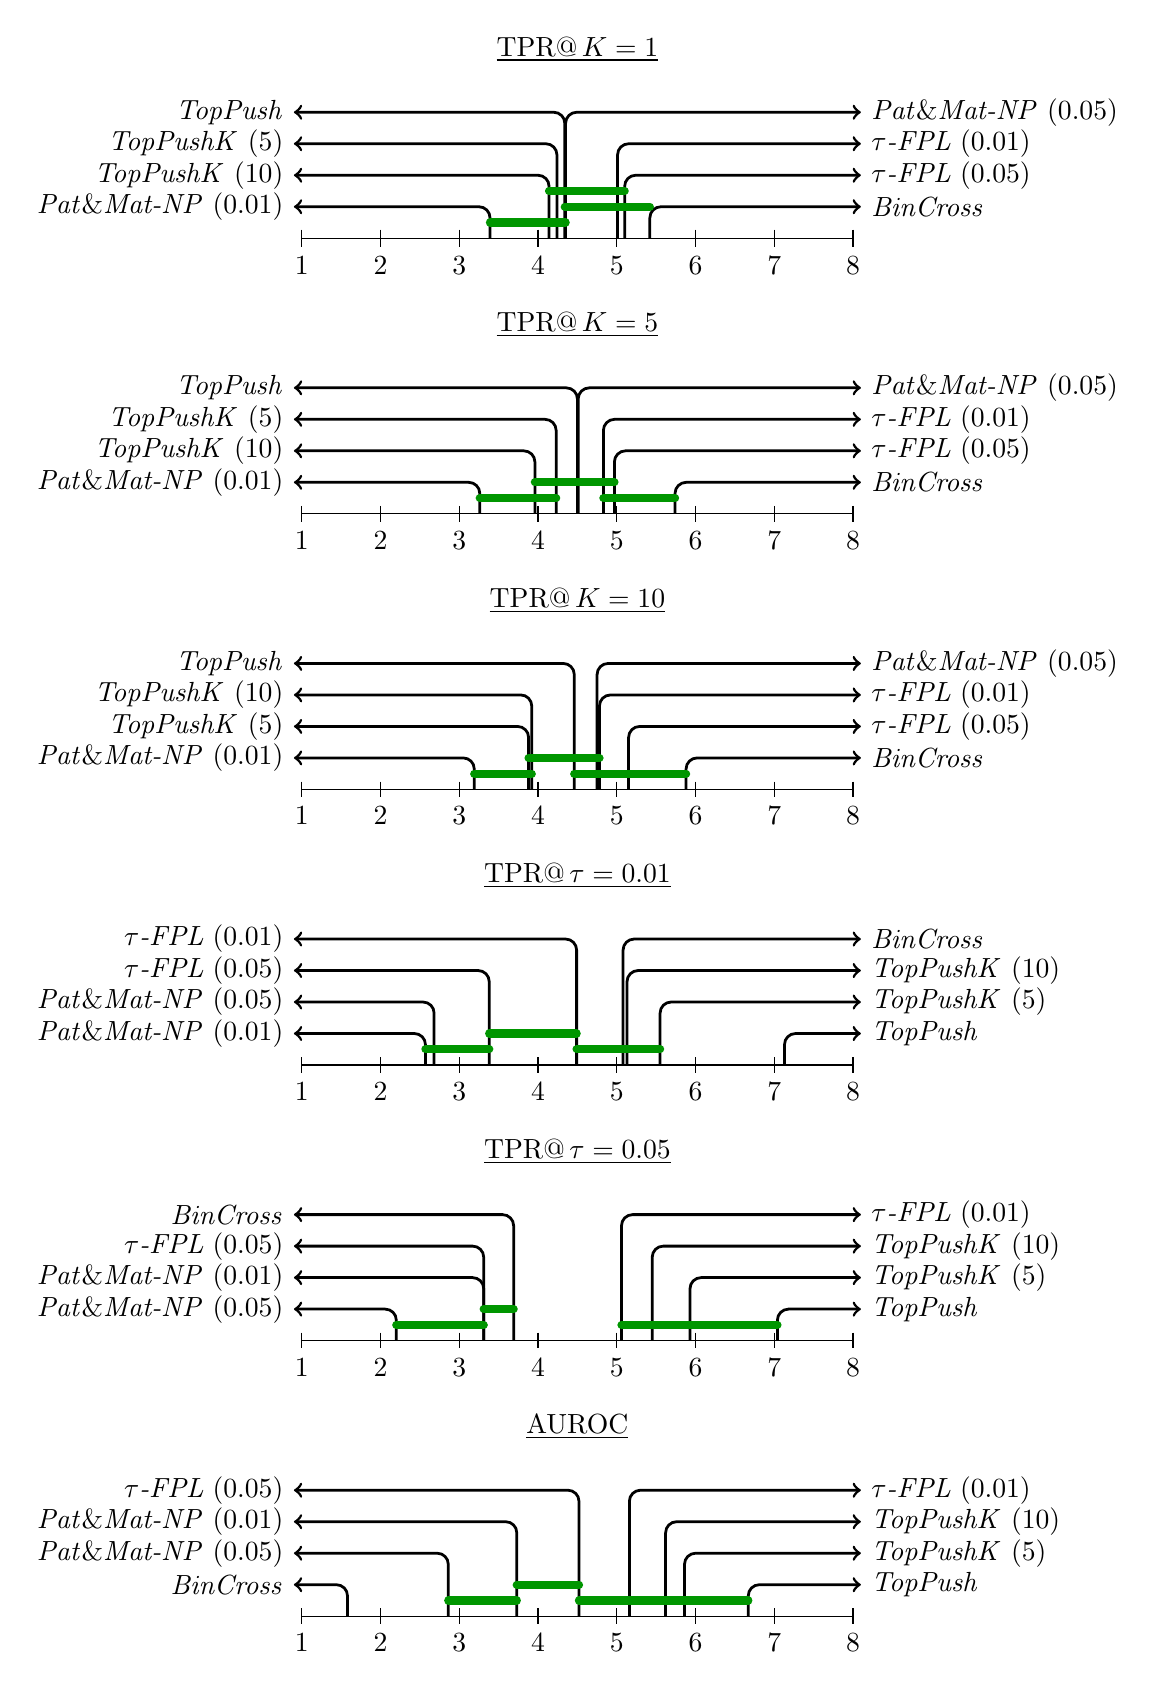
\begin{tikzpicture}  \node at (4.5,2.4) {\underline{$\auroc$}}; 
  \draw (1,0) -- (8,0); 
  \foreach \x in {1,...,8} \draw (\x,0.1) -- (\x,-0.1) node[anchor=north]{$\x$}; 
  \draw[line_node] (1.58,0) -- (1.58,0.4) -- (0.9, 0.4) node[anchor=east] {\BaseLine}; 
  \draw[line_node] (2.86,0) -- (2.86,0.8) -- (0.9, 0.8) node[anchor=east] {\PatMatNP(0.05)}; 
  \draw[line_node] (3.73,0) -- (3.73,1.2) -- (0.9, 1.2) node[anchor=east] {\PatMatNP(0.01)}; 
  \draw[line_node] (4.52,0) -- (4.52,1.6) -- (0.9, 1.6) node[anchor=east] {\tauFPL(0.05)}; 
  \draw[line_node] (5.16,0) -- (5.16,1.6) -- (8.1, 1.6) node[anchor=west] {\tauFPL(0.01)}; 
  \draw[line_node] (5.62,0) -- (5.62,1.2) -- (8.1, 1.2) node[anchor=west] {\TopPushK(10)}; 
  \draw[line_node] (5.86,0) -- (5.86,0.8) -- (8.1, 0.8) node[anchor=west] {\TopPushK(5)}; 
  \draw[line_node] (6.67,0) -- (6.67,0.4) -- (8.1, 0.4) node[anchor=west] {\TopPush}; 
  \draw[line_cv] (2.86,0.2) -- (3.73, 0.2); 
  \draw[line_cv] (3.73,0.4) -- (4.52, 0.4); 
  \draw[line_cv] (4.52,0.2) -- (5.62, 0.2); 
  \draw[line_cv] (5.16,0.2) -- (5.86, 0.2); 
  \draw[line_cv] (5.62,0.2) -- (6.67, 0.2); 


  \node at (4.5,5.9) {\underline{$\tpratfpr = 0.05$}}; 
  \draw (1,3.5) -- (8,3.5); 
  \foreach \x in {1,...,8} \draw (\x,3.6) -- (\x,3.4) node[anchor=north]{$\x$}; 
  \draw[line_node] (2.2,3.5) -- (2.2,3.9) -- (0.9, 3.9) node[anchor=east] {\PatMatNP(0.05)}; 
  \draw[line_node] (3.31,3.5) -- (3.31,4.3) -- (0.9, 4.3) node[anchor=east] {\PatMatNP(0.01)}; 
  \draw[line_node] (3.31,3.5) -- (3.31,4.7) -- (0.9, 4.7) node[anchor=east] {\tauFPL(0.05)}; 
  \draw[line_node] (3.69,3.5) -- (3.69,5.1) -- (0.9, 5.1) node[anchor=east] {\BaseLine}; 
  \draw[line_node] (5.06,3.5) -- (5.06,5.1) -- (8.1, 5.1) node[anchor=west] {\tauFPL(0.01)}; 
  \draw[line_node] (5.45,3.5) -- (5.45,4.7) -- (8.1, 4.7) node[anchor=west] {\TopPushK(10)}; 
  \draw[line_node] (5.93,3.5) -- (5.93,4.3) -- (8.1, 4.3) node[anchor=west] {\TopPushK(5)}; 
  \draw[line_node] (7.04,3.5) -- (7.04,3.9) -- (8.1, 3.9) node[anchor=west] {\TopPush}; 
  \draw[line_cv] (2.2,3.7) -- (3.31, 3.7); 
  \draw[line_cv] (3.31,3.9) -- (3.69, 3.9); 
  \draw[line_cv] (5.06,3.7) -- (5.93, 3.7); 
  \draw[line_cv] (5.93,3.7) -- (7.04, 3.7); 


  \node at (4.5,9.4) {\underline{$\tpratfpr = 0.01$}}; 
  \draw (1,7.0) -- (8,7.0); 
  \foreach \x in {1,...,8} \draw (\x,7.1) -- (\x,6.9) node[anchor=north]{$\x$}; 
  \draw[line_node] (2.57,7.0) -- (2.57,7.4) -- (0.9, 7.4) node[anchor=east] {\PatMatNP(0.01)}; 
  \draw[line_node] (2.68,7.0) -- (2.68,7.8) -- (0.9, 7.8) node[anchor=east] {\PatMatNP(0.05)}; 
  \draw[line_node] (3.38,7.0) -- (3.38,8.2) -- (0.9, 8.2) node[anchor=east] {\tauFPL(0.05)}; 
  \draw[line_node] (4.49,7.0) -- (4.49,8.6) -- (0.9, 8.6) node[anchor=east] {\tauFPL(0.01)}; 
  \draw[line_node] (5.08,7.0) -- (5.08,8.6) -- (8.1, 8.6) node[anchor=west] {\BaseLine}; 
  \draw[line_node] (5.13,7.0) -- (5.13,8.2) -- (8.1, 8.2) node[anchor=west] {\TopPushK(10)}; 
  \draw[line_node] (5.55,7.0) -- (5.55,7.8) -- (8.1, 7.8) node[anchor=west] {\TopPushK(5)}; 
  \draw[line_node] (7.13,7.0) -- (7.13,7.4) -- (8.1, 7.4) node[anchor=west] {\TopPush}; 
  \draw[line_cv] (2.57,7.2) -- (3.38, 7.2); 
  \draw[line_cv] (3.38,7.4) -- (4.49, 7.4); 
  \draw[line_cv] (4.49,7.2) -- (5.55, 7.2); 


  \node at (4.5,12.9) {\underline{$\tpratk =10$}}; 
  \draw (1,10.5) -- (8,10.5); 
  \foreach \x in {1,...,8} \draw (\x,10.6) -- (\x,10.4) node[anchor=north]{$\x$}; 
  \draw[line_node] (3.19,10.5) -- (3.19,10.9) -- (0.9, 10.9) node[anchor=east] {\PatMatNP(0.01)}; 
  \draw[line_node] (3.88,10.5) -- (3.88,11.3) -- (0.9, 11.3) node[anchor=east] {\TopPushK(5)}; 
  \draw[line_node] (3.92,10.5) -- (3.92,11.7) -- (0.9, 11.7) node[anchor=east] {\TopPushK(10)}; 
  \draw[line_node] (4.46,10.5) -- (4.46,12.1) -- (0.9, 12.1) node[anchor=east] {\TopPush}; 
  \draw[line_node] (4.75,10.5) -- (4.75,12.1) -- (8.1, 12.1) node[anchor=west] {\PatMatNP(0.05)}; 
  \draw[line_node] (4.78,10.5) -- (4.78,11.7) -- (8.1, 11.7) node[anchor=west] {\tauFPL(0.01)}; 
  \draw[line_node] (5.15,10.5) -- (5.15,11.3) -- (8.1, 11.3) node[anchor=west] {\tauFPL(0.05)}; 
  \draw[line_node] (5.88,10.5) -- (5.88,10.9) -- (8.1, 10.9) node[anchor=west] {\BaseLine}; 
  \draw[line_cv] (3.19,10.7) -- (3.92, 10.7); 
  \draw[line_cv] (3.88,10.9) -- (4.78, 10.9); 
  \draw[line_cv] (4.46,10.7) -- (5.15, 10.7); 
  \draw[line_cv] (4.75,10.7) -- (5.88, 10.7); 


  \node at (4.5,16.4) {\underline{$\tpratk =5$}}; 
  \draw (1,14.0) -- (8,14.0); 
  \foreach \x in {1,...,8} \draw (\x,14.1) -- (\x,13.9) node[anchor=north]{$\x$}; 
  \draw[line_node] (3.26,14.0) -- (3.26,14.4) -- (0.9, 14.4) node[anchor=east] {\PatMatNP(0.01)}; 
  \draw[line_node] (3.96,14.0) -- (3.96,14.8) -- (0.9, 14.8) node[anchor=east] {\TopPushK(10)}; 
  \draw[line_node] (4.23,14.0) -- (4.23,15.2) -- (0.9, 15.2) node[anchor=east] {\TopPushK(5)}; 
  \draw[line_node] (4.5,14.0) -- (4.5,15.6) -- (0.9, 15.6) node[anchor=east] {\TopPush}; 
  \draw[line_node] (4.51,14.0) -- (4.51,15.6) -- (8.1, 15.6) node[anchor=west] {\PatMatNP(0.05)}; 
  \draw[line_node] (4.83,14.0) -- (4.83,15.2) -- (8.1, 15.2) node[anchor=west] {\tauFPL(0.01)}; 
  \draw[line_node] (4.97,14.0) -- (4.97,14.8) -- (8.1, 14.8) node[anchor=west] {\tauFPL(0.05)}; 
  \draw[line_node] (5.74,14.0) -- (5.74,14.4) -- (8.1, 14.4) node[anchor=west] {\BaseLine}; 
  \draw[line_cv] (3.26,14.2) -- (4.23, 14.2); 
  \draw[line_cv] (3.96,14.4) -- (4.97, 14.4); 
  \draw[line_cv] (4.83,14.2) -- (5.74, 14.2); 


  \node at (4.5,19.9) {\underline{$\tpratk =1$}}; 
  \draw (1,17.5) -- (8,17.5); 
  \foreach \x in {1,...,8} \draw (\x,17.61) -- (\x,17.39) node[anchor=north]{$\x$}; 
  \draw[line_node] (3.39,17.5) -- (3.39,17.9) -- (0.9, 17.9) node[anchor=east] {\PatMatNP(0.01)}; 
  \draw[line_node] (4.14,17.5) -- (4.14,18.3) -- (0.9, 18.3) node[anchor=east] {\TopPushK(10)}; 
  \draw[line_node] (4.24,17.5) -- (4.24,18.7) -- (0.9, 18.7) node[anchor=east] {\TopPushK(5)}; 
  \draw[line_node] (4.34,17.5) -- (4.34,19.1) -- (0.9, 19.1) node[anchor=east] {\TopPush}; 
  \draw[line_node] (4.35,17.5) -- (4.35,19.1) -- (8.1, 19.1) node[anchor=west] {\PatMatNP(0.05)}; 
  \draw[line_node] (5.01,17.5) -- (5.01,18.7) -- (8.1, 18.7) node[anchor=west] {\tauFPL(0.01)}; 
  \draw[line_node] (5.1,17.5) -- (5.1,18.3) -- (8.1, 18.3) node[anchor=west] {\tauFPL(0.05)}; 
  \draw[line_node] (5.42,17.5) -- (5.42,17.9) -- (8.1, 17.9) node[anchor=west] {\BaseLine}; 
  \draw[line_cv] (3.39,17.7) -- (4.35, 17.7); 
  \draw[line_cv] (4.14,18.1) -- (5.1, 18.1); 
  \draw[line_cv] (4.34,17.9) -- (5.42, 17.9); 
\end{tikzpicture}

  \caption{\textbf{Primal formulation with linear model:} Critical difference (CD) diagrams (level of importance 0.05) of the Nemenyi post hoc test for the Friedman test. Each diagram shows the mean rank of each method, with rank 1 being the best. Green wide horizontal lines group together methods with the mean ranks that are not significantly different. The critical difference diagrams were computed for mean rank averages over all datasets.}
  \label{fig: critical diagrams primal}
\end{figure}

\newpage

\subsection{Dual Formulation: Linear Model}\label{sec: results dual}

\begin{table}[!p]
  \centering
  \underline{$\tpratk =10$}
  \vspace{0.25cm}\\
  \resizebox{\columnwidth}{!}{% 
    \begin{NiceTabular}{lcccccc}
      \CodeBefore
        \rowcolor{\headercol}{1}
        \rowcolors{3}{\rowcol}{}[restart]
      \Body
      \toprule
      \textbf{Formulation}
        & \textbf{MNIST}
        & \textbf{FashionMNIST}
        & \textbf{CIFAR10}
        & \textbf{CIFAR20}
        & \textbf{CIFAR100}
        & \textbf{SVHN2}\\
      \midrule
      \SVM
        & 97.89
        & \best{95.40}
        & 9.10
        & 4.90
        & \best{11.50}
        & 4.52 \\
      \TopPush
        & 97.62
        & 94.80
        & 10.45
        & \best{6.10}
        & 11.00
        & 5.23 \\
      \TopPushK(5)
        & 97.97
        & 94.90
        & 10.05
        & 6.00
        & 11.0
        & 5.07 \\
      \TopPushK(10)
        & 97.97
        & 94.90
        & 9.85
        & \best{6.10}
        & 11.00
        & 5.18 \\
      \tauFPL(0.01)
        & \best{98.02}
        & 95.05
        & \best{10.70}
        & 5.90
        & 10.5
        & \best{5.25} \\
      \tauFPL(0.05)
        & 92.56
        & \worst{92.20}
        & 10.15
        & 5.10
        & 10.0
        & 5.24 \\
      \PatMatNP(0.01)
        & 88.37
        & 92.50
        & \worst{7.45}
        & 1.40
        & \worst{5.00}
        & \worst{4.02} \\
      \PatMatNP(0.05)
        & \worst{52.60}
        & 92.50
        & \worst{7.45}
        & \worst{1.30}
        & \worst{5.00}
        & 4.05 \\
      \bottomrule
    \end{NiceTabular}
  }
  \vspace{0.25cm}\\
  \underline{$\tpratfpr = 0.05$}
  \vspace{0.25cm}\\
  \resizebox{\columnwidth}{!}{% 
    \begin{NiceTabular}{lcccccc}
      \CodeBefore
        \rowcolor{\headercol}{1}
        \rowcolors{3}{\rowcol}{}[restart]
      \Body
      \toprule
      \textbf{Formulation}
        & \textbf{MNIST}
        & \textbf{FashionMNIST}
        & \textbf{CIFAR10}
        & \textbf{CIFAR20}
        & \textbf{CIFAR100}
        & \textbf{SVHN2}\\
      \midrule
      \SVM
        & 99.74
        & 98.90
        & 60.00
        & \best{44.80}
        & 59.00
        & \worst{59.72} \\
      \TopPush
        & 99.74
        & 98.80
        & 57.10
        & \worst{37.70}
        & 59.50
        & 72.54 \\
      \TopPushK(5)
        & \best{99.82}
        & 98.90
        & 56.25
        & 38.80
        & \worst{57.50}
        & 71.40 \\
      \TopPushK(10)
        & \best{99.82}
        & 98.90
        & 56.90
        & 38.70
        & 58.00
        & 71.61 \\
      \tauFPL(0.01)
        & \best{99.82}
        & 98.90
        & 58.10
        & 39.10
        & 59.00
        & 73.52 \\
      \tauFPL(0.05)
        & 99.74
        & \best{99.10}
        & \best{60.80}
        & 44.40
        & 61.00
        & \best{74.26} \\
      \PatMatNP(0.01)
        & \worst{99.30}
        & \worst{98.10}
        & \worst{54.70}
        & 44.60
        & 62.50
        & 63.47 \\
      \PatMatNP(0.05)
        & 99.38
        & \worst{98.10}
        & \worst{54.70}
        & 44.50
        & \best{63.50}
        & 63.48 \\
      \bottomrule
    \end{NiceTabular}
  }
  \vspace{0.25cm}\\
  \underline{$\auroc$}
  \vspace{0.25cm}\\
  \resizebox{\columnwidth}{!}{% 
    \begin{NiceTabular}{lcccccc}
      \CodeBefore
        \rowcolor{\headercol}{1}
        \rowcolors{3}{\rowcol}{}[restart]
      \Body
      \toprule
      \textbf{Formulation}
        & \textbf{MNIST}
        & \textbf{FashionMNIST}
        & \textbf{CIFAR10}
        & \textbf{CIFAR20}
        & \textbf{CIFAR100}
        & \textbf{SVHN2}\\
      \midrule
      \SVM
        & 99.94
        & 99.66
        & 90.02
        & 79.75
        & 87.80
        & \worst{90.14} \\
      \TopPush
        & 99.94
        & 99.56
        & 89.35
        & 79.06
        & \worst{87.03}
        & 92.77 \\
      \TopPushK(5)
        & 99.95
        & 99.64
        & 89.05
        & 79.13
        & 87.21
        & 92.60 \\
      \TopPushK(10)
        & 99.95
        & 99.67
        & 89.16
        & 79.27
        & 87.78
        & 92.67 \\
      \tauFPL(0.01)
        & \best{99.97}
        & 99.68
        & 89.83
        & 79.07
        & 87.64
        & 92.98 \\
      \tauFPL(0.05)
        & 99.93
        & \best{99.80}
        & \best{90.34}
        & \best{80.17}
        & 88.56
        & \best{93.16} \\
      \PatMatNP(0.01)
        & \worst{99.78}
        & \worst{99.40}
        & 87.62
        & 78.82
        & \best{89.78}
        & 90.80 \\
      \PatMatNP(0.05)
        & \worst{99.78}
        & \worst{99.40}
        & \worst{87.61}
        & \worst{78.76}
        & 89.52
        & 90.82 \\
      \bottomrule
    \end{NiceTabular}
  }
  \caption{\textbf{Dual formulations with gaussian kernel:} Each table corresponds to one performance metric and all presented results are medians of ten independent runs for each pair of datasets and formulation. The best result for each dataset is highlighted in green, while the worst result is highlighted in red.}
  \label{tab: dual auc}
\end{table}

\begin{figure}[!p]
  \centering
  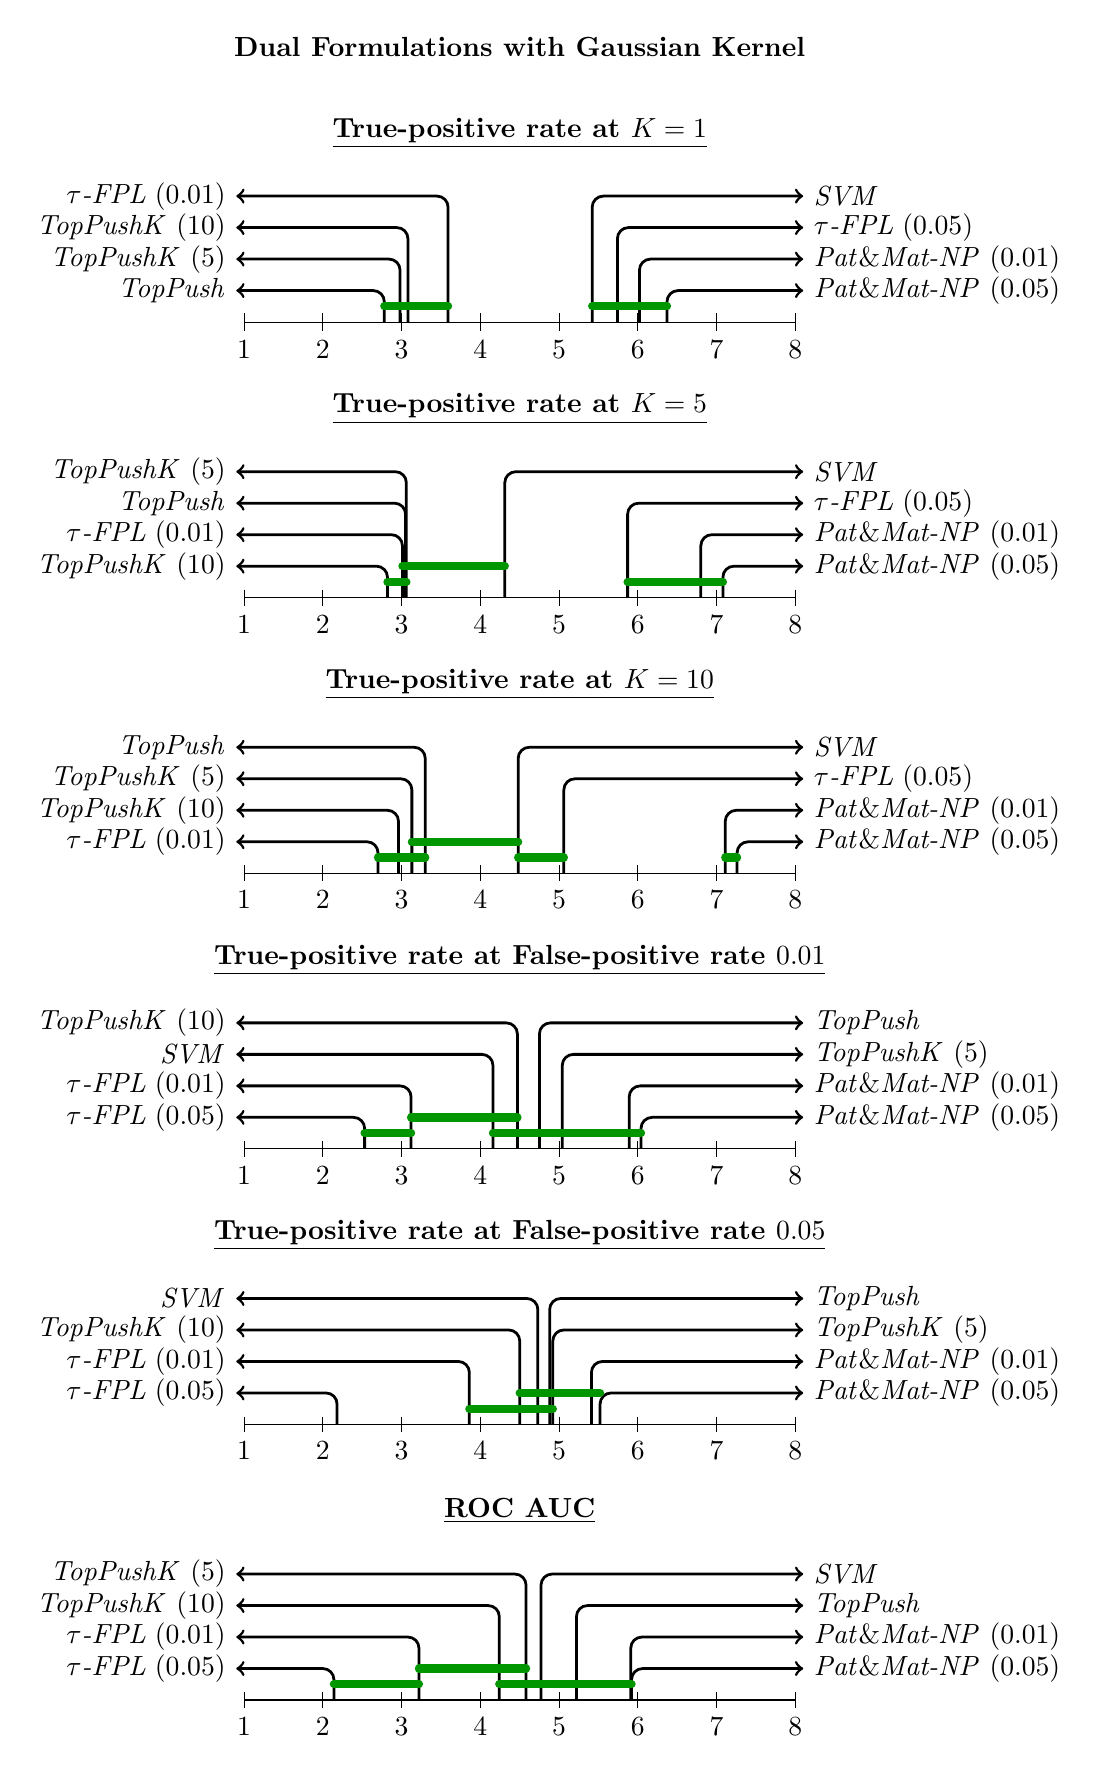
\begin{tikzpicture}  \node at (4.5,2.4) {\textbf{\underline{ROC AUC}}}; 
  \draw (1,0) -- (8,0); 
  \foreach \x in {1,...,8} \draw (\x,0.1) -- (\x,-0.1) node[anchor=north]{$\x$}; 
  \draw[line_node] (2.14,0) -- (2.14,0.4) -- (0.9, 0.4) node[anchor=east] {\tauFPL(0.05)}; 
  \draw[line_node] (3.22,0) -- (3.22,0.8) -- (0.9, 0.8) node[anchor=east] {\tauFPL(0.01)}; 
  \draw[line_node] (4.24,0) -- (4.24,1.2) -- (0.9, 1.2) node[anchor=east] {\TopPushK(10)}; 
  \draw[line_node] (4.58,0) -- (4.58,1.6) -- (0.9, 1.6) node[anchor=east] {\TopPushK(5)}; 
  \draw[line_node] (4.77,0) -- (4.77,1.6) -- (8.1, 1.6) node[anchor=west] {\SVM}; 
  \draw[line_node] (5.22,0) -- (5.22,1.2) -- (8.1, 1.2) node[anchor=west] {\TopPush}; 
  \draw[line_node] (5.91,0) -- (5.91,0.8) -- (8.1, 0.8) node[anchor=west] {\PatMatNP(0.01)}; 
  \draw[line_node] (5.92,0) -- (5.92,0.4) -- (8.1, 0.4) node[anchor=west] {\PatMatNP(0.05)}; 
  \draw[line_cv] (2.14,0.2) -- (3.22, 0.2); 
  \draw[line_cv] (3.22,0.4) -- (4.58, 0.4); 
  \draw[line_cv] (4.24,0.2) -- (5.22, 0.2); 
  \draw[line_cv] (4.58,0.2) -- (5.92, 0.2); 


  \node at (4.5,5.9) {\textbf{\underline{True-positive rate at False-positive rate $0.05$}}}; 
  \draw (1,3.5) -- (8,3.5); 
  \foreach \x in {1,...,8} \draw (\x,3.6) -- (\x,3.4) node[anchor=north]{$\x$}; 
  \draw[line_node] (2.18,3.5) -- (2.18,3.9) -- (0.9, 3.9) node[anchor=east] {\tauFPL(0.05)}; 
  \draw[line_node] (3.86,3.5) -- (3.86,4.3) -- (0.9, 4.3) node[anchor=east] {\tauFPL(0.01)}; 
  \draw[line_node] (4.5,3.5) -- (4.5,4.7) -- (0.9, 4.7) node[anchor=east] {\TopPushK(10)}; 
  \draw[line_node] (4.73,3.5) -- (4.73,5.1) -- (0.9, 5.1) node[anchor=east] {\SVM}; 
  \draw[line_node] (4.88,3.5) -- (4.88,5.1) -- (8.1, 5.1) node[anchor=west] {\TopPush}; 
  \draw[line_node] (4.92,3.5) -- (4.92,4.7) -- (8.1, 4.7) node[anchor=west] {\TopPushK(5)}; 
  \draw[line_node] (5.41,3.5) -- (5.41,4.3) -- (8.1, 4.3) node[anchor=west] {\PatMatNP(0.01)}; 
  \draw[line_node] (5.52,3.5) -- (5.52,3.9) -- (8.1, 3.9) node[anchor=west] {\PatMatNP(0.05)}; 
  \draw[line_cv] (3.86,3.7) -- (4.92, 3.7); 
  \draw[line_cv] (4.5,3.9) -- (5.52, 3.9); 


  \node at (4.5,9.4) {\textbf{\underline{True-positive rate at False-positive rate $0.01$}}}; 
  \draw (1,7.0) -- (8,7.0); 
  \foreach \x in {1,...,8} \draw (\x,7.1) -- (\x,6.9) node[anchor=north]{$\x$}; 
  \draw[line_node] (2.53,7.0) -- (2.53,7.4) -- (0.9, 7.4) node[anchor=east] {\tauFPL(0.05)}; 
  \draw[line_node] (3.12,7.0) -- (3.12,7.8) -- (0.9, 7.8) node[anchor=east] {\tauFPL(0.01)}; 
  \draw[line_node] (4.16,7.0) -- (4.16,8.2) -- (0.9, 8.2) node[anchor=east] {\SVM}; 
  \draw[line_node] (4.47,7.0) -- (4.47,8.6) -- (0.9, 8.6) node[anchor=east] {\TopPushK(10)}; 
  \draw[line_node] (4.75,7.0) -- (4.75,8.6) -- (8.1, 8.6) node[anchor=west] {\TopPush}; 
  \draw[line_node] (5.04,7.0) -- (5.04,8.2) -- (8.1, 8.2) node[anchor=west] {\TopPushK(5)}; 
  \draw[line_node] (5.89,7.0) -- (5.89,7.8) -- (8.1, 7.8) node[anchor=west] {\PatMatNP(0.01)}; 
  \draw[line_node] (6.04,7.0) -- (6.04,7.4) -- (8.1, 7.4) node[anchor=west] {\PatMatNP(0.05)}; 
  \draw[line_cv] (2.53,7.2) -- (3.12, 7.2); 
  \draw[line_cv] (3.12,7.4) -- (4.47, 7.4); 
  \draw[line_cv] (4.16,7.2) -- (5.04, 7.2); 
  \draw[line_cv] (4.75,7.2) -- (6.04, 7.2); 


  \node at (4.5,12.9) {\textbf{\underline{True-positive rate at $K = 10$}}}; 
  \draw (1,10.5) -- (8,10.5); 
  \foreach \x in {1,...,8} \draw (\x,10.6) -- (\x,10.4) node[anchor=north]{$\x$}; 
  \draw[line_node] (2.7,10.5) -- (2.7,10.9) -- (0.9, 10.9) node[anchor=east] {\tauFPL(0.01)}; 
  \draw[line_node] (2.96,10.5) -- (2.96,11.3) -- (0.9, 11.3) node[anchor=east] {\TopPushK(10)}; 
  \draw[line_node] (3.13,10.5) -- (3.13,11.7) -- (0.9, 11.7) node[anchor=east] {\TopPushK(5)}; 
  \draw[line_node] (3.3,10.5) -- (3.3,12.1) -- (0.9, 12.1) node[anchor=east] {\TopPush}; 
  \draw[line_node] (4.48,10.5) -- (4.48,12.1) -- (8.1, 12.1) node[anchor=west] {\SVM}; 
  \draw[line_node] (5.06,10.5) -- (5.06,11.7) -- (8.1, 11.7) node[anchor=west] {\tauFPL(0.05)}; 
  \draw[line_node] (7.11,10.5) -- (7.11,11.3) -- (8.1, 11.3) node[anchor=west] {\PatMatNP(0.01)}; 
  \draw[line_node] (7.26,10.5) -- (7.26,10.9) -- (8.1, 10.9) node[anchor=west] {\PatMatNP(0.05)}; 
  \draw[line_cv] (2.7,10.7) -- (3.3, 10.7); 
  \draw[line_cv] (3.13,10.9) -- (4.48, 10.9); 
  \draw[line_cv] (4.48,10.7) -- (5.06, 10.7); 
  \draw[line_cv] (7.11,10.7) -- (7.26, 10.7); 


  \node at (4.5,16.4) {\textbf{\underline{True-positive rate at $K = 5$}}}; 
  \draw (1,14.0) -- (8,14.0); 
  \foreach \x in {1,...,8} \draw (\x,14.1) -- (\x,13.9) node[anchor=north]{$\x$}; 
  \draw[line_node] (2.82,14.0) -- (2.82,14.4) -- (0.9, 14.4) node[anchor=east] {\TopPushK(10)}; 
  \draw[line_node] (3.01,14.0) -- (3.01,14.8) -- (0.9, 14.8) node[anchor=east] {\tauFPL(0.01)}; 
  \draw[line_node] (3.05,14.0) -- (3.05,15.2) -- (0.9, 15.2) node[anchor=east] {\TopPush}; 
  \draw[line_node] (3.06,14.0) -- (3.06,15.6) -- (0.9, 15.6) node[anchor=east] {\TopPushK(5)}; 
  \draw[line_node] (4.31,14.0) -- (4.31,15.6) -- (8.1, 15.6) node[anchor=west] {\SVM}; 
  \draw[line_node] (5.87,14.0) -- (5.87,15.2) -- (8.1, 15.2) node[anchor=west] {\tauFPL(0.05)}; 
  \draw[line_node] (6.8,14.0) -- (6.8,14.8) -- (8.1, 14.8) node[anchor=west] {\PatMatNP(0.01)}; 
  \draw[line_node] (7.08,14.0) -- (7.08,14.4) -- (8.1, 14.4) node[anchor=west] {\PatMatNP(0.05)}; 
  \draw[line_cv] (2.82,14.2) -- (3.06, 14.2); 
  \draw[line_cv] (3.01,14.4) -- (4.31, 14.4); 
  \draw[line_cv] (5.87,14.2) -- (7.08, 14.2); 


  \node at (4.5,19.9) {\textbf{\underline{True-positive rate at $K = 1$}}}; 
  \draw (1,17.5) -- (8,17.5); 
  \foreach \x in {1,...,8} \draw (\x,17.61) -- (\x,17.39) node[anchor=north]{$\x$}; 
  \draw[line_node] (2.78,17.5) -- (2.78,17.9) -- (0.9, 17.9) node[anchor=east] {\TopPush}; 
  \draw[line_node] (2.98,17.5) -- (2.98,18.3) -- (0.9, 18.3) node[anchor=east] {\TopPushK(5)}; 
  \draw[line_node] (3.08,17.5) -- (3.08,18.7) -- (0.9, 18.7) node[anchor=east] {\TopPushK(10)}; 
  \draw[line_node] (3.59,17.5) -- (3.59,19.1) -- (0.9, 19.1) node[anchor=east] {\tauFPL(0.01)}; 
  \draw[line_node] (5.42,17.5) -- (5.42,19.1) -- (8.1, 19.1) node[anchor=west] {\SVM}; 
  \draw[line_node] (5.74,17.5) -- (5.74,18.7) -- (8.1, 18.7) node[anchor=west] {\tauFPL(0.05)}; 
  \draw[line_node] (6.02,17.5) -- (6.02,18.3) -- (8.1, 18.3) node[anchor=west] {\PatMatNP(0.01)}; 
  \draw[line_node] (6.37,17.5) -- (6.37,17.9) -- (8.1, 17.9) node[anchor=west] {\PatMatNP(0.05)}; 
  \draw[line_cv] (2.78,17.7) -- (3.59, 17.7); 
  \draw[line_cv] (5.42,17.7) -- (6.37, 17.7); 


\node at (4.5, 21.0) {\textbf{Dual Formulations with Gaussian Kernel}}; 
\end{tikzpicture}

  \caption{\textbf{Dual formulations with gaussian kernel:} Critical difference (CD) diagrams (level of importance 0.05) of the Nemenyi post hoc test for the Friedman test. Each diagram shows the mean rank of each method, with rank 1 being the best. Green wide horizontal lines group together methods with the mean ranks that are not significantly different. The critical difference diagrams were computed for mean rank averages over all datasets.}
  \label{fig: critical diagrams dual gauss}
\end{figure}

\newpage

\subsection{Primal Formulation: Non-Linear Model}\label{sec: results primal nonlinear}

In this subsection, we discuss result for the case of primal formulations with linear model, i.e. resutls presented here are related to the Chapter~\ref{chap: linear}.

\begin{table}[!p]
  \centering
  \underline{$\tpratk =10$}
  \vspace{0.25cm}\\
  \resizebox{\columnwidth}{!}{% 
    \begin{NiceTabular}{lccccccc}
      \CodeBefore
        \rowcolor{\headercol}{1}
        \rowcolors{3}{\rowcol}{}[restart]
      \Body
      \toprule
      \textbf{Formulation}
        & \textbf{MNIST}
        & \textbf{FashionMNIST}
        & \textbf{CIFAR10}
        & \textbf{CIFAR20}
        & \textbf{CIFAR100}
        & \textbf{SVHN2}
        & \textbf{SVHN2Extra}\\
      \midrule
      \BaseLine
        & \best{99.26}
        & \best{98.10}
        & 11.40
        & 3.50
        & 5.00
        & 11.34
        & 15.95 \\
      \DeepTopPush
        & 98.42
        & 97.60
        & \worst{0.20}
        & 0.20
        & \worst{0.00}
        & \worst{0.17}
        & \worst{0.00} \\
      \TopPushK(5)
        & 98.54
        & 97.50
        & 2.00
        & \worst{0.00}
        & 8.50
        & 10.58
        & 16.12 \\
      \TopPushK(10)
        & 98.24
        & 96.90
        & 12.55
        & \best{100.00}
        & \best{100.00}
        & \best{100.00}
        & \best{100.00} \\
      \tauFPL(0.01)
        & 98.72
        & 97.50
        & 1.00
        & 0.20
        & 9.00
        & 9.52
        & \worst{0.00} \\
      \tauFPL(0.05)
        & 96.78
        & 96.50
        & 14.80
        & 0.30
        & 8.50
        & 13.05
        & 12.48 \\
      \PatMatNP(0.01)
        & 98.54
        & 97.45
        & \best{32.45}
        & 4.80
        & 20.00
        & 13.92
        & 19.33 \\
      \PatMatNP(0.05)
        & \worst{82.86}
        & \worst{94.30}
        & 26.55
        & 5.90
        & 11.50
        & 11.36
        & 15.98 \\
      \bottomrule
    \end{NiceTabular}
  }
  \vspace{0.25cm}\\
  \underline{$\tpratfpr = 0.05$}
  \vspace{0.25cm}\\
  \resizebox{\columnwidth}{!}{% 
    \begin{NiceTabular}{lccccccc}
      \CodeBefore
        \rowcolor{\headercol}{1}
        \rowcolors{3}{\rowcol}{}[restart]
      \Body
      \toprule
      \textbf{Formulation}
        & \textbf{MNIST}
        & \textbf{FashionMNIST}
        & \textbf{CIFAR10}
        & \textbf{CIFAR20}
        & \textbf{CIFAR100}
        & \textbf{SVHN2}
        & \textbf{SVHN2Extra}\\
      \midrule
      \BaseLine
        & \best{100.00}
        & \best{99.90}
        & 83.35
        & 48.00
        & 82.00
        & 94.66
        & 97.71 \\
      \DeepTopPush
        & \worst{99.82}
        & \worst{99.70}
        & \worst{5.85}
        & 8.90
        & 9.00
        & 40.14
        & \worst{0.00} \\
      \TopPushK(5)
        & \best{100.00}
        & 99.85
        & 34.30
        & 7.70
        & 53.50
        & 86.54
        & 93.96 \\
      \TopPushK(10)
        & \best{100.00}
        & \best{99.90}
        & 27.95
        & \worst{0.00}
        & \worst{0.00}
        & \worst{0.00}
        & \worst{0.00} \\
      \tauFPL(0.01)
        & \best{100.00}
        & \best{99.90}
        & 24.40
        & 11.50
        & 65.50
        & 87.60
        & \worst{0.00} \\
      \tauFPL(0.05)
        & \best{100.00}
        & \best{99.90}
        & 82.75
        & 18.00
        & 66.50
        & 94.51
        & 97.52 \\
      \PatMatNP(0.01)
        & \best{100.00}
        & \best{99.90}
        & 91.55
        & 52.20
        & 79.00
        & 95.49
        & 98.43 \\
      \PatMatNP(0.05)
        & \best{100.00}
        & \best{99.90}
        & \best{91.75}
        & \best{57.70}
        & \best{85.00}
        & \best{95.53}
        & \best{98.50} \\
      \bottomrule
    \end{NiceTabular}
  }
  \vspace{0.25cm}\\
  \underline{$\auroc$}
  \vspace{0.25cm}\\
  \resizebox{\columnwidth}{!}{% 
    \begin{NiceTabular}{lccccccc}
      \CodeBefore
        \rowcolor{\headercol}{1}
        \rowcolors{3}{\rowcol}{}[restart]
      \Body
      \toprule
      \textbf{Formulation}
        & \textbf{MNIST}
        & \textbf{FashionMNIST}
        & \textbf{CIFAR10}
        & \textbf{CIFAR20}
        & \textbf{CIFAR100}
        & \textbf{SVHN2}
        & \textbf{SVHN2Extra}\\
      \midrule
      \BaseLine
        & \best{100.00}
        & \best{99.98}
        & 96.85
        & 84.67
        & 95.94
        & 98.54
        & 99.20 \\
      \DeepTopPush
        & 99.98
        & \worst{99.95}
        & \worst{49.51}
        & 59.40
        & 56.68
        & 83.12
        & 1.61 \\
      \TopPushK(5)
        & \best{100.0}
        & 99.97
        & 77.10
        & 55.50
        & 84.24
        & 96.57
        & 98.32 \\
      \TopPushK(10)
        & \best{100.00}
        & \best{99.98}
        & 74.26
        & \worst{0.00}
        & \worst{0.00}
        & \worst{0.00}
        & \worst{0.00} \\
      \tauFPL(0.01)
        & \best{100.0}
        & \best{99.98}
        & 70.96
        & 60.03
        & 90.16
        & 96.68
        & 25.84 \\
      \tauFPL(0.05)
        & 99.99
        & 99.97
        & 95.86
        & 68.18
        & 90.76
        & 98.50
        & 99.12 \\
      \PatMatNP(0.01)
        & 99.99
        & \best{99.98}
        & 97.90
        & 84.38
        & 93.84
        & 98.74
        & \best{99.38} \\
      \PatMatNP(0.05)
        & \worst{99.96}
        & 99.96
        & \best{98.24}
        & \best{88.39}
        & \best{96.56}
        & \best{98.76}
        & 99.32 \\
      \bottomrule
    \end{NiceTabular}
  }
  \caption{\textbf{Primal formulations with non-linear model:} Each table corresponds to one performance metric and all presented results are medians of ten independent runs for each pair of datasets and formulation. The best result for each dataset is highlighted in green, while the worst result is highlighted in red.}
  \label{tab: primalnn auc}
\end{table}

\begin{figure}[!p]
  \centering
  \documentclass{standalone}
% ------------------------------------------------------------------------------
% Packages
% ------------------------------------------------------------------------------
\usepackage[ddmmyyyy]{datetime}
\usepackage[T1]{fontenc}
\usepackage[utf8]{inputenc}

% Page setting
\usepackage[explicit]{titlesec}
\usepackage{sectsty}
\usepackage{fancyhdr}
\usepackage[title, titletoc]{appendix}

% Fonts
\usepackage{kpfonts}
\usepackage{amsmath}
\usepackage{amssymb}
\usepackage{dsfont}
\usepackage{pifont}

% Graphics and colors
\usepackage{graphicx}
\usepackage{xcolor}
\usepackage{import}

\definecolor{myred}{RGB}{150,0,0}
\definecolor{mygreen}{RGB}{0,150,0}
\definecolor{myblue}{RGB}{0, 101, 189}
\definecolor{myyellow}{RGB}{220, 206, 0}
\definecolor{myorange}{RGB}{255, 153, 51}
\definecolor{mycyan}{RGB}{51, 204, 204}
\definecolor{mypurple}{RGB}{204, 0, 153}

\newcommand{\doccol}{\color{myblue}}

% Hyperrefs
\usepackage[
  pdfusetitle,
  unicode = true,
  bookmarks = true,
  bookmarksnumbered = false,
  bookmarksopen = true,
  breaklinks = false,
  pdfborderstyle = {},
  backref = false,
  colorlinks = true,
  linkcolor = myblue,
  urlcolor = myred,
  citecolor = mygreen,
]{hyperref}


% Captions
\usepackage{caption}

\captionsetup[figure]{position = bottom}
\captionsetup[table]{position = bottom}

% Tables, Algs ...
\usepackage{enumitem}
\usepackage{algorithm}
\usepackage{algorithmicx}
\usepackage{algpseudocode}
\usepackage{booktabs}
\usepackage{nicematrix}

\renewcommand{\arraystretch}{1.5}

\newcommand{\headercol}{myblue!20}
\newcommand{\rowcol}{myblue!10}

% Math
\usepackage{nicefrac}
\usepackage{bm}
\usepackage{thm-restate}
\usepackage{optidef}
\usepackage{xspace}

% Theorems
\usepackage[framemethod=TikZ]{mdframed}
\usepackage{amsthm}
\usepackage{xifthen}

% Tikz and pfgplots
\usepackage{tikz}
\usepackage{pgfplots}
\usepackage{pgfplotstable}

\usetikzlibrary{shapes}
\usetikzlibrary{arrows}
\usetikzlibrary{automata}
\usetikzlibrary{positioning}
\usetikzlibrary{calc}
\usetikzlibrary{intersections}

\pgfplotsset{compat=newest}
\usepgfplotslibrary{groupplots}
\usepgfplotslibrary{fillbetween}

\tikzstyle{line_node} = [line width=1pt, rounded corners, color=black, ->]
\tikzstyle{line_cv} = [line width=3pt, color=mygreen, line cap=round]

% Tmp
\usepackage[color=myred!50]{todonotes}

% ------------------------------------------------------------------------------
% Math declarations
% ------------------------------------------------------------------------------
\newcommand{\Brac}[2][r]{%
  \ifx r#1 \left(       #2 \right)       \else
  \ifx c#1 \left\{      #2 \right\}      \else
  \ifx s#1 \left[       #2 \right]       \else
  \ifx v#1 \left\vert   #2 \right\vert   \else
  \ifx a#1 \left\langle #2 \right\rangle \else
  \ifx t#1 \left\lceil  #2 \right\rceil  \else
  \ifx b#1 \left\lfloor #2 \right\rfloor \else
  \ifx n#1 \left\|      #2 \right\|      \else
  \mathrm{Illegal~option}%
  \fi\fi\fi\fi\fi\fi\fi\fi
}

\newcommand{\clip}[4][s]{
  \ifx s#1 \mathrm{clip}_{\Brac[s]{#2,\; #3}}\Brac{#4} \else
  \ifx u#1 \mathrm{clip}_{\left[#2,\; #3\right)}\Brac{#4} \else
  \ifx l#1 \mathrm{clip}_{\left(#2,\; #3\right]}\Brac{#4} \else
  \mathrm{Illegal~option}%
  \fi\fi\fi
}

\DeclareMathOperator*{\argmax}{arg\,max}

\newcommand{\yesmark}{\textcolor{mygreen}{\ding{51}}}%
\newcommand{\nomark}{\textcolor{myred}{\ding{55}}}
\newcommand{\good}[1]{\textcolor{mygreen}{#1}}
\newcommand{\bad}[1]{\textcolor{myred}{#1}}

\newcommand{\R}{\mathbb{R}}
\newcommand{\N}{\mathbb{N}}
\newcommand{\X}{\mathbb{X}}

\newcommand{\I}{\mathcal{I}}
\newcommand{\Itil}{\tilde{\mathcal{I}}}
\newcommand{\Ineg}{\I_{-}}
\newcommand{\Ipos}{\I_{+}}

\newcommand{\Imb}{\I_{\text{mb}}}
\newcommand{\Imbneg}{\I_{\text{mb},-}}
\newcommand{\Imbpos}{\I_{\text{mb},+}}

\newcommand{\indmax}{j^{\star}}
\newcommand{\indmaxmb}{j^{\star}_{\text{mb}}}

\newcommand{\nall}{n}
\newcommand{\nneg}{n_{-}}
\newcommand{\npos}{n_{+}}
\newcommand{\ntil}{\tilde{n}}

\newcommand{\nmb}{n_{\text{mb}}}
\newcommand{\nmbneg}{n_{\text{mb},-}}
\newcommand{\nmbpos}{n_{\text{mb},+}}

\newcommand{\K}{\mathbb{K}}
\newcommand{\Kall}{\K^{\pm}}
\newcommand{\Kneg}{\K^{-}}

\newcommand{\alphak}{\alpha_{\hat{k}}}
\newcommand{\alphal}{\alpha_{\hat{l}}}
\newcommand{\betak}{\beta_{\hat{k}}}
\newcommand{\betal}{\beta_{\hat{l}}}

\newcommand{\norm}[1]{\Brac[n]{#1}}
\newcommand{\abs}[1]{|#1|}
\newcommand{\inner}[2]{\Brac[a]{#1, \; #2}}
\newcommand{\dd}[1]{\mathop{}\!\mathrm{d}#1}

\newcommand{\Iverson}[1]{\mathds{1}_{\Brac[s]{#1}}}

\newcommand{\EE}{\mathbb{E}}
\newcommand{\PP}{\mathbb{P}}
\newcommand{\bias}{\operatorname{bias}}

\newcommand{\Matrix}[1]{\begin{pmatrix} #1 \end{pmatrix}}
\newcommand{\Set}[2]{\Brac[c]{#1 \; \middle\vert \; #2}}
\newcommand{\domain}{\operatorname*{dom}}

\newcommand{\repeatloop}{\texttt{repeat}\xspace}
\newcommand{\forloop}{\texttt{for}\xspace}

\newcommand{\vecab}{\Matrix{\bm{\alpha} \\ \bm{\beta}}}

% models
\newcommand{\AccatTop}{\emph{Accuracy at the Top}\xspace}
\newcommand{\TopPush}{\emph{TopPush}\xspace}
\newcommand{\TopPushK}{\emph{TopPushK}\xspace}
\newcommand{\tauFPL}{{\emph{$\tau$-FPL}}\xspace}
\newcommand{\TopMeanK}{\emph{TopMeanK}\xspace}
\newcommand{\PatMat}{\emph{Pat}\&\emph{Mat}\xspace}
\newcommand{\PatMatNP}{{\emph{Pat}\&\emph{Mat-NP}}\xspace}
\newcommand{\Grill}{\emph{Grill}\xspace}
\newcommand{\GrillNP}{\emph{Grill-NP}\xspace}
\newcommand{\DeepTopPush}{\emph{DeepTopPush}\xspace}
\newcommand{\TFCO}{\emph{TFCO}\xspace}
\newcommand{\APPerf}{\emph{Ap-Perf}\xspace}
\newcommand{\BaseLine}{\emph{BinCross}\xspace}
\newcommand{\SVM}{\emph{SVM}\xspace}

% counts and rates
\DeclareMathOperator{\tp}{tp}
\DeclareMathOperator{\tn}{tn}
\DeclareMathOperator{\fp}{fp}
\DeclareMathOperator{\fn}{fn}
\DeclareMathOperator{\tpr}{tpr}
\DeclareMathOperator{\tnr}{tnr}
\DeclareMathOperator{\fpr}{fpr}
\DeclareMathOperator{\fnr}{fnr}

\DeclareMathOperator{\tps}{\overline{tp}}
\DeclareMathOperator{\tns}{\overline{tn}}
\DeclareMathOperator{\fps}{\overline{fp}}
\DeclareMathOperator{\fns}{\overline{fn}}

\DeclareMathOperator{\accuracy}{acc}
\DeclareMathOperator{\baccuracy}{bacc}
\DeclareMathOperator{\precision}{precision}
\DeclareMathOperator{\recall}{recall}
\DeclareMathOperator{\pratrec}{Precision@Recall}
\DeclareMathOperator{\postop}{pos@top}

\newcommand{\tpratk}{\operatorname{TPR@}K}
\newcommand{\tpratfpr}{\operatorname{TPR@}\tau}
\newcommand{\auroc}{\operatorname{AUROC}}


% ------------------------------------------------------------------------------
% Document
% ------------------------------------------------------------------------------
\tikzstyle{line_node} = [line width=1pt, rounded corners, color=black, ->]
\tikzstyle{line_cv} = [line width=3pt, color=mygreen, line cap=round]

\begin{document}
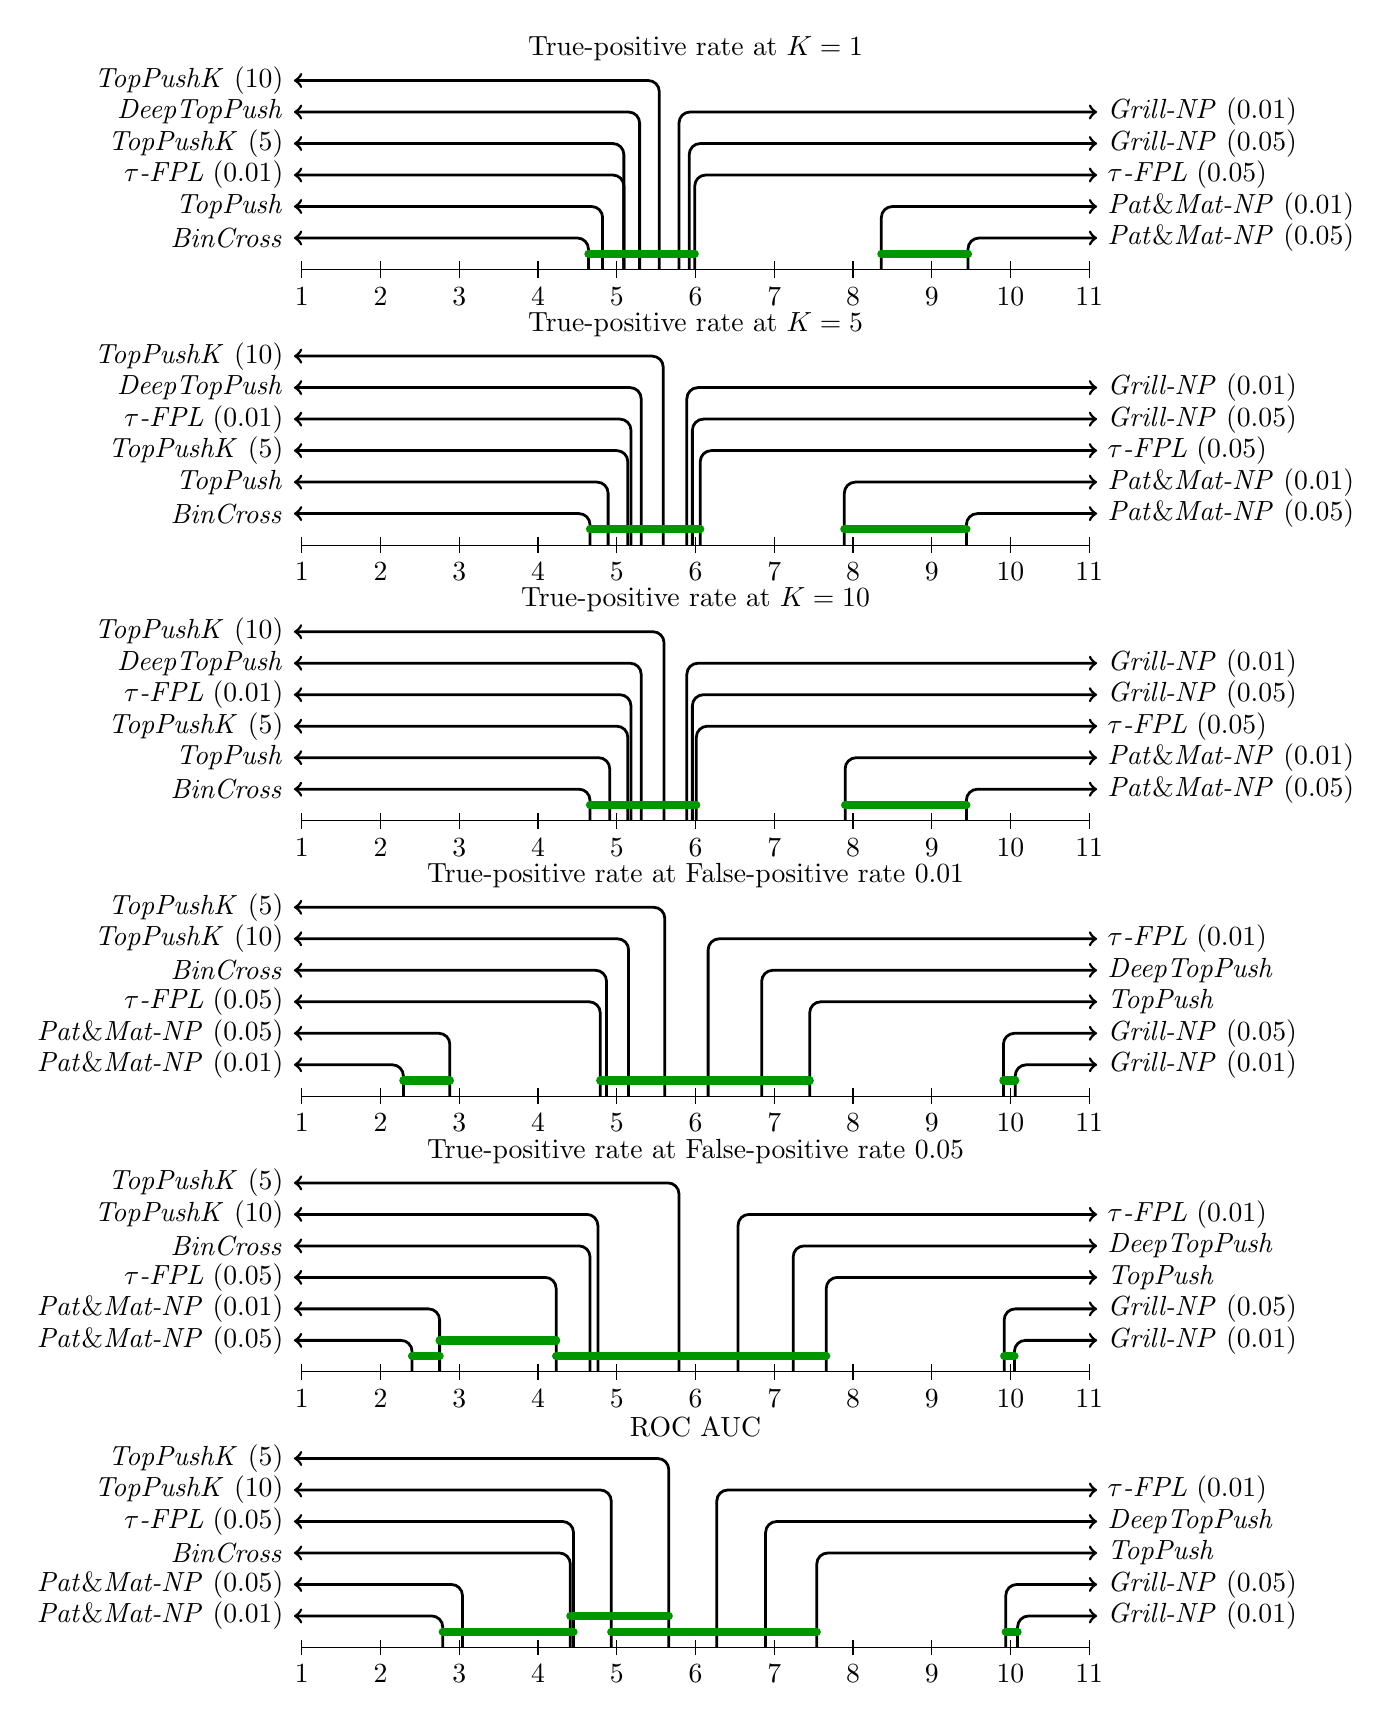
\begin{tikzpicture}
  \node at (6.0,2.8) {ROC AUC}; 
  \draw (1,0) -- (11,0); 
  \foreach \x in {1,...,11} \draw (\x,0.1) -- (\x,-0.1) node[anchor=north]{$\x$}; 
  \draw[line_node] (2.79,0) -- (2.79,0.4) -- (0.9, 0.4) node[anchor=east] {\PatMatNP(0.01)}; 
  \draw[line_node] (3.04,0) -- (3.04,0.8) -- (0.9, 0.8) node[anchor=east] {\PatMatNP(0.05)}; 
  \draw[line_node] (4.41,0) -- (4.41,1.2) -- (0.9, 1.2) node[anchor=east] {\BaseLine}; 
  \draw[line_node] (4.45,0) -- (4.45,1.6) -- (0.9, 1.6) node[anchor=east] {\tauFPL(0.05)}; 
  \draw[line_node] (4.93,0) -- (4.93,2.0) -- (0.9, 2.0) node[anchor=east] {\TopPushK(10)}; 
  \draw[line_node] (5.66,0) -- (5.66,2.4) -- (0.9, 2.4) node[anchor=east] {\TopPushK(5)}; 
  \draw[line_node] (6.27,0) -- (6.27,2.0) -- (11.1, 2.0) node[anchor=west] {\tauFPL(0.01)}; 
  \draw[line_node] (6.89,0) -- (6.89,1.6) -- (11.1, 1.6) node[anchor=west] {\DeepTopPush}; 
  \draw[line_node] (7.54,0) -- (7.54,1.2) -- (11.1, 1.2) node[anchor=west] {\TopPush}; 
  \draw[line_node] (9.94,0) -- (9.94,0.8) -- (11.1, 0.8) node[anchor=west] {\GrillNP(0.05)}; 
  \draw[line_node] (10.09,0) -- (10.09,0.4) -- (11.1, 0.4) node[anchor=west] {\GrillNP(0.01)}; 
  \draw[line_cv] (2.79,0.2) -- (4.45, 0.2); 
  \draw[line_cv] (4.41,0.4) -- (5.66, 0.4); 
  \draw[line_cv] (4.93,0.2) -- (6.27, 0.2); 
  \draw[line_cv] (5.66,0.2) -- (6.89, 0.2); 
  \draw[line_cv] (6.27,0.2) -- (7.54, 0.2); 
  \draw[line_cv] (9.94,0.2) -- (10.09, 0.2); 

  \node at (6.0,6.3) {True-positive rate at False-positive rate $0.05$}; 
  \draw (1,3.5) -- (11,3.5); 
  \foreach \x in {1,...,11} \draw (\x,3.6) -- (\x,3.4) node[anchor=north]{$\x$}; 
  \draw[line_node] (2.4,3.5) -- (2.4,3.9) -- (0.9, 3.9) node[anchor=east] {\PatMatNP(0.05)}; 
  \draw[line_node] (2.75,3.5) -- (2.75,4.3) -- (0.9, 4.3) node[anchor=east] {\PatMatNP(0.01)}; 
  \draw[line_node] (4.23,3.5) -- (4.23,4.7) -- (0.9, 4.7) node[anchor=east] {\tauFPL(0.05)}; 
  \draw[line_node] (4.66,3.5) -- (4.66,5.1) -- (0.9, 5.1) node[anchor=east] {\BaseLine}; 
  \draw[line_node] (4.76,3.5) -- (4.76,5.5) -- (0.9, 5.5) node[anchor=east] {\TopPushK(10)}; 
  \draw[line_node] (5.79,3.5) -- (5.79,5.9) -- (0.9, 5.9) node[anchor=east] {\TopPushK(5)}; 
  \draw[line_node] (6.54,3.5) -- (6.54,5.5) -- (11.1, 5.5) node[anchor=west] {\tauFPL(0.01)}; 
  \draw[line_node] (7.24,3.5) -- (7.24,5.1) -- (11.1, 5.1) node[anchor=west] {\DeepTopPush}; 
  \draw[line_node] (7.66,3.5) -- (7.66,4.7) -- (11.1, 4.7) node[anchor=west] {\TopPush}; 
  \draw[line_node] (9.92,3.5) -- (9.92,4.3) -- (11.1, 4.3) node[anchor=west] {\GrillNP(0.05)}; 
  \draw[line_node] (10.05,3.5) -- (10.05,3.9) -- (11.1, 3.9) node[anchor=west] {\GrillNP(0.01)}; 
  \draw[line_cv] (2.4,3.7) -- (2.75, 3.7); 
  \draw[line_cv] (2.75,3.9) -- (4.23, 3.9); 
  \draw[line_cv] (4.23,3.7) -- (5.79, 3.7); 
  \draw[line_cv] (4.76,3.7) -- (6.54, 3.7); 
  \draw[line_cv] (5.79,3.7) -- (7.24, 3.7); 
  \draw[line_cv] (6.54,3.7) -- (7.66, 3.7); 
  \draw[line_cv] (9.92,3.7) -- (10.05, 3.7); 

  \node at (6.0,9.8) {True-positive rate at False-positive rate $0.01$}; 
  \draw (1,7.0) -- (11,7.0); 
  \foreach \x in {1,...,11} \draw (\x,7.1) -- (\x,6.9) node[anchor=north]{$\x$}; 
  \draw[line_node] (2.29,7.0) -- (2.29,7.4) -- (0.9, 7.4) node[anchor=east] {\PatMatNP(0.01)}; 
  \draw[line_node] (2.88,7.0) -- (2.88,7.8) -- (0.9, 7.8) node[anchor=east] {\PatMatNP(0.05)}; 
  \draw[line_node] (4.79,7.0) -- (4.79,8.2) -- (0.9, 8.2) node[anchor=east] {\tauFPL(0.05)}; 
  \draw[line_node] (4.87,7.0) -- (4.87,8.6) -- (0.9, 8.6) node[anchor=east] {\BaseLine}; 
  \draw[line_node] (5.15,7.0) -- (5.15,9.0) -- (0.9, 9.0) node[anchor=east] {\TopPushK(10)}; 
  \draw[line_node] (5.61,7.0) -- (5.61,9.4) -- (0.9, 9.4) node[anchor=east] {\TopPushK(5)}; 
  \draw[line_node] (6.16,7.0) -- (6.16,9.0) -- (11.1, 9.0) node[anchor=west] {\tauFPL(0.01)}; 
  \draw[line_node] (6.84,7.0) -- (6.84,8.6) -- (11.1, 8.6) node[anchor=west] {\DeepTopPush}; 
  \draw[line_node] (7.45,7.0) -- (7.45,8.2) -- (11.1, 8.2) node[anchor=west] {\TopPush}; 
  \draw[line_node] (9.91,7.0) -- (9.91,7.8) -- (11.1, 7.8) node[anchor=west] {\GrillNP(0.05)}; 
  \draw[line_node] (10.06,7.0) -- (10.06,7.4) -- (11.1, 7.4) node[anchor=west] {\GrillNP(0.01)}; 
  \draw[line_cv] (2.29,7.2) -- (2.88, 7.2); 
  \draw[line_cv] (4.79,7.2) -- (6.16, 7.2); 
  \draw[line_cv] (5.15,7.2) -- (6.84, 7.2); 
  \draw[line_cv] (6.16,7.2) -- (7.45, 7.2); 
  \draw[line_cv] (9.91,7.2) -- (10.06, 7.2); 

  \node at (6.0,13.3) {True-positive rate at $K = 10$}; 
  \draw (1,10.5) -- (11,10.5); 
  \foreach \x in {1,...,11} \draw (\x,10.6) -- (\x,10.4) node[anchor=north]{$\x$}; 
  \draw[line_node] (4.66,10.5) -- (4.66,10.9) -- (0.9, 10.9) node[anchor=east] {\BaseLine}; 
  \draw[line_node] (4.91,10.5) -- (4.91,11.3) -- (0.9, 11.3) node[anchor=east] {\TopPush}; 
  \draw[line_node] (5.14,10.5) -- (5.14,11.7) -- (0.9, 11.7) node[anchor=east] {\TopPushK(5)}; 
  \draw[line_node] (5.18,10.5) -- (5.18,12.1) -- (0.9, 12.1) node[anchor=east] {\tauFPL(0.01)}; 
  \draw[line_node] (5.31,10.5) -- (5.31,12.5) -- (0.9, 12.5) node[anchor=east] {\DeepTopPush}; 
  \draw[line_node] (5.6,10.5) -- (5.6,12.9) -- (0.9, 12.9) node[anchor=east] {\TopPushK(10)}; 
  \draw[line_node] (5.89,10.5) -- (5.89,12.5) -- (11.1, 12.5) node[anchor=west] {\GrillNP(0.01)}; 
  \draw[line_node] (5.96,10.5) -- (5.96,12.1) -- (11.1, 12.1) node[anchor=west] {\GrillNP(0.05)}; 
  \draw[line_node] (6.01,10.5) -- (6.01,11.7) -- (11.1, 11.7) node[anchor=west] {\tauFPL(0.05)}; 
  \draw[line_node] (7.9,10.5) -- (7.9,11.3) -- (11.1, 11.3) node[anchor=west] {\PatMatNP(0.01)}; 
  \draw[line_node] (9.44,10.5) -- (9.44,10.9) -- (11.1, 10.9) node[anchor=west] {\PatMatNP(0.05)}; 
  \draw[line_cv] (4.66,10.7) -- (6.01, 10.7); 
  \draw[line_cv] (7.9,10.7) -- (9.44, 10.7); 

  \node at (6.0,16.8) {True-positive rate at $K = 5$}; 
  \draw (1,14.0) -- (11,14.0); 
  \foreach \x in {1,...,11} \draw (\x,14.1) -- (\x,13.9) node[anchor=north]{$\x$}; 
  \draw[line_node] (4.66,14.0) -- (4.66,14.4) -- (0.9, 14.4) node[anchor=east] {\BaseLine}; 
  \draw[line_node] (4.89,14.0) -- (4.89,14.8) -- (0.9, 14.8) node[anchor=east] {\TopPush}; 
  \draw[line_node] (5.14,14.0) -- (5.14,15.2) -- (0.9, 15.2) node[anchor=east] {\TopPushK(5)}; 
  \draw[line_node] (5.18,14.0) -- (5.18,15.6) -- (0.9, 15.6) node[anchor=east] {\tauFPL(0.01)}; 
  \draw[line_node] (5.31,14.0) -- (5.31,16.0) -- (0.9, 16.0) node[anchor=east] {\DeepTopPush}; 
  \draw[line_node] (5.59,14.0) -- (5.59,16.4) -- (0.9, 16.4) node[anchor=east] {\TopPushK(10)}; 
  \draw[line_node] (5.89,14.0) -- (5.89,16.0) -- (11.1, 16.0) node[anchor=west] {\GrillNP(0.01)}; 
  \draw[line_node] (5.96,14.0) -- (5.96,15.6) -- (11.1, 15.6) node[anchor=west] {\GrillNP(0.05)}; 
  \draw[line_node] (6.06,14.0) -- (6.06,15.2) -- (11.1, 15.2) node[anchor=west] {\tauFPL(0.05)}; 
  \draw[line_node] (7.89,14.0) -- (7.89,14.8) -- (11.1, 14.8) node[anchor=west] {\PatMatNP(0.01)}; 
  \draw[line_node] (9.44,14.0) -- (9.44,14.4) -- (11.1, 14.4) node[anchor=west] {\PatMatNP(0.05)}; 
  \draw[line_cv] (4.66,14.2) -- (6.06, 14.2); 
  \draw[line_cv] (7.89,14.2) -- (9.44, 14.2); 

  \node at (6.0,20.3) {True-positive rate at $K = 1$}; 
  \draw (1,17.5) -- (11,17.5); 
  \foreach \x in {1,...,11} \draw (\x,17.61) -- (\x,17.39) node[anchor=north]{$\x$}; 
  \draw[line_node] (4.64,17.5) -- (4.64,17.9) -- (0.9, 17.9) node[anchor=east] {\BaseLine}; 
  \draw[line_node] (4.82,17.5) -- (4.82,18.3) -- (0.9, 18.3) node[anchor=east] {\TopPush}; 
  \draw[line_node] (5.09,17.5) -- (5.09,18.7) -- (0.9, 18.7) node[anchor=east] {\tauFPL(0.01)}; 
  \draw[line_node] (5.09,17.5) -- (5.09,19.1) -- (0.9, 19.1) node[anchor=east] {\TopPushK(5)}; 
  \draw[line_node] (5.29,17.5) -- (5.29,19.5) -- (0.9, 19.5) node[anchor=east] {\DeepTopPush}; 
  \draw[line_node] (5.54,17.5) -- (5.54,19.9) -- (0.9, 19.9) node[anchor=east] {\TopPushK(10)}; 
  \draw[line_node] (5.79,17.5) -- (5.79,19.5) -- (11.1, 19.5) node[anchor=west] {\GrillNP(0.01)}; 
  \draw[line_node] (5.92,17.5) -- (5.92,19.1) -- (11.1, 19.1) node[anchor=west] {\GrillNP(0.05)}; 
  \draw[line_node] (5.99,17.5) -- (5.99,18.7) -- (11.1, 18.7) node[anchor=west] {\tauFPL(0.05)}; 
  \draw[line_node] (8.36,17.5) -- (8.36,18.3) -- (11.1, 18.3) node[anchor=west] {\PatMatNP(0.01)}; 
  \draw[line_node] (9.46,17.5) -- (9.46,17.9) -- (11.1, 17.9) node[anchor=west] {\PatMatNP(0.05)}; 
  \draw[line_cv] (4.64,17.7) -- (5.99, 17.7); 
  \draw[line_cv] (8.36,17.7) -- (9.46, 17.7); 
\end{tikzpicture}
\end{document}

  \caption{\textbf{Primal formulations with non-linear model:} Critical difference (CD) diagrams (level of importance 0.05) of the Nemenyi post hoc test for the Friedman test. Each diagram shows the mean rank of each method, with rank 1 being the best. Green wide horizontal lines group together methods with the mean ranks that are not significantly different. The critical difference diagrams were computed for mean rank averages over all datasets.}
  \label{fig: critical diagrams primal NN}
\end{figure}

\newpage

\section{Steganalysis}\label{sec: steganalysis}

In the previous section, we presented results on standard image recognition datasets. Even though the results are quite good even on these datasets, they did not fully show the importance of the problem of classification at the top. To show the importance of this problem properly,  we need to find the field in which the maximizing true-positive rate at the low false-positive rate is an important task. Such a field can be for example steganography and steganalysis. The standard way how to share secret information these days is the use of encryption. However, in such a case, the presence of a secret message (even though encrypted) is obvious. Steganography aims to hide the fact that communication taking place, by hiding the secret message within an ordinary file (usually called cover file) in order to avoid detection. The secret message is then extracted at its destination. The secret data can be hidden in almost any type of digital content, however the most popular are images. There are two reasons for this. The first of them is the ubiquity of images on the Internet and therefore the ease to use them as cover files for secret messages. The second reason is their large potential payload, i.e. it is possible to hide a lot of information in the images with high resolution. With an appropriate cover image and steganography tools, it is possible to create an stego-image (image with a hidden message) that can not be recognized from the cover image by human perception. However, each tool leaves a fingerprint or signature in the image, that can be used to detect stego images. The field that tries to detect stego images and possibly decrypt messages from them is called steganalysis. In steganalysis, the goal is to achieve the best true-positive rate with the lowest possible false-positive rate. Therefore steganalysis is the branch suitable for the classification at the top, since many of the formulations derived in this work focus precisely on this task. \cite{morkel2005overview, silman2001steganography} 

For the eperiments, we have a large dataset of cover-images that consists of approximately 450 000 images from Flickr. All these images are in the JPEG format with quality factor 80. Since the dataset does not contain any stego images, we use two different ways to generate them. For the purpose of this work, we named them \textbf{Nsf5} and \textbf{JMiPOD}.

\subsection{Nsf5}

In this case, we generate stego images using simulated F5 with matrix embedding turned off and we use payload 0.2. Since we are interested in low false-positive rates, we need a lot of negative (cover) samples to estimate it. This is evident in~\eqref{eq: patmat np} where the threshold~$t$ is a surrogate approximation of false-positive rate, i.e., the threshold is computed only from negative samples. Positive (stego) samples occurs only in the objective function. Since generating of stego images is expensive and we do not need them to estimate false-positive rate, we decided to use 10\% of all cover images to generate their stego counterparts. All images (both cover and stego images) are then described using 22 500 features and split into train / validation / test set in ratio 0.45 / 0.05 / 0.5. The resulting sizes of train / validation / test splits as well as the number of stego images in them, are in Table~\ref{tab: datasets summary}. 

Since the resulting classification task is relatively easier to solve, we decided to use a simple linear model. The number o training samples and their size is not too big, therefore we can load the whole dataset into memory. It allows us to use full gradient descent instead of its stochastic version. As an optimizer, we use the ADAM~\cite{kingma2014adam} with default settings and fixed step length~$\alpha = 0.01.$ We also use a fixed number of epochs to 1000 for all formulations. Finally, we repeat each experiment ten times with ten different random seeds.

Figure~\ref{fig: steganalysis nsf5} shows ROC curves for the test set of \textbf{Nsf5} dataset. For simplicity, we show ROC curves only for one run of the experiment. Moreover, Table~\ref{tab: steganalysis nsf5} shows seven different performance metrics computed for each formulation. Each shown result in this table is a median of ten independent runs. It is evident, that \BaseLine provides very poor results for all metrics except the $\auroc$. Surprisingly, \BaseLine is the worst even for the $\auroc.$ On the other hand, \DeepTopPush excels at very low false-positive rates, as can be seen from both the table and the figure. In fact, \DeepTopPush provides the best results for four out of seven performance metrics (the best results are highlighted in green). Note that all these four metrics operate at extremely small false-positive rates. We can also see, that \PatMatNP($10^{-5}$) is the best at false-positive rate~$10^{-4}$. This unexpected result is probably caused by the approximation of the true top $\tau$-quantile of all scores of negative samples in \PatMatNP formulation. Therefore, \PatMatNP($10^{-5}$) is optimized for a false-positive rate slightly higher than~$10^{-5}$ and as a consequence outperforms \PatMatNP($10^{-5}$) at false-positive rate~$10^{-4}$. Similar behavior can be seen for \PatMatNP($10^{-4}$) and \PatMatNP($10^{-3}$) at false-positive rate~$10^{-4}$.

\begin{figure}
  \centering
  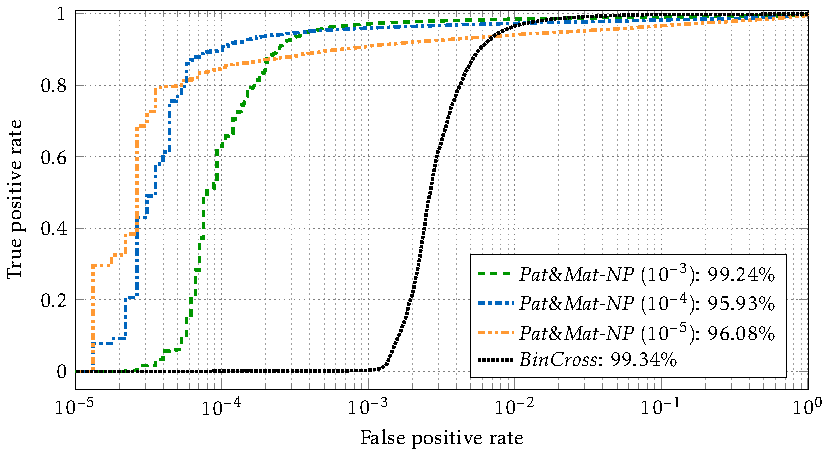
\includegraphics{images/stego_nsft5.pdf}
  \caption{\textbf{Nsf5 dataset:} ROC curves with logaithmic $x$-axis.}
  \label{fig: steganalysis nsf5}
\end{figure}

\begin{table}[!t]
  \centering
  \begin{NiceTabular}{lccccccc}
    \CodeBefore
    \rowcolor{\headercol}{1-2}
    \rowcolors{4}{\rowcol}{}[restart]
    \Body
    \toprule
    \Block[c]{2-1}{\textbf{Formulation}}
    & \Block[c]{2-1}{$\auroc$}
    & \Block[c]{1-3}{$\tpratk$}
    &&& \Block[c]{1-3}{$\tpratfpr$} \\
    \cline{3-8}
    && $1$
    & $10$
    & $5$
    & $10^{-5}$
    & $10^{-4}$
    & $10^{-3}$ \\
    \midrule
    \BaseLine
    & \worst{95.84}
    & \worst{0.0}
    & \worst{0.0}
    & \worst{0.0}
    & \worst{0.0}
    & \worst{0.02}
    & \worst{0.7} \\
    \DeepTopPush
    & 98.29
    & \best{5.07}
    & \best{35.48}
    & \best{57.66}
    & \best{48.65}
    & 89.56
    & 93.67 \\
    \PatMatNP($10^{-5}$)
    & 98.81
    & 2.55
    & 23.02
    & 47.24
    & 35.28
    & \best{91.9}
    & 95.84 \\
    \PatMatNP($10^{-4}$)
    & 98.98
    & \worst{0.0}
    & 0.05
    & 4.34
    & 1.78
    & 79.76
    & \best{96.18} \\
    \PatMatNP($10^{-3}$)
    & \best{99.26}
    & \worst{0.0}
    & \worst{0.0}
    & 0.01
    & \worst{0.0}
    & 0.29
    & 91.98 \\
    \bottomrule
  \end{NiceTabular}
  \caption{\textbf{NSF5 dataset:}  All presented results are medians of ten independent runs with different random seeds. Each column of the table corresponds to one performance metric and every row to one formulation. The best result for each metric is highlighted in green, while the worst result is highlighted in red.}
  \label{tab: steganalysis nsf5}
\end{table}

\subsection{JMiPOD}

In this case, we first select all images that can be cropped to to size $256 \times 256 \times 3$ and than cropped them looselesly using \emph{jpegtran} library. Than, we use JMiPOD~\cite{cogranne2020steganography} algorithm to generate stego images with payload 0.1. We use the same approach as in the case of Nsf5 dataset and use only 10\% of cover images to generate their stego counterparts. We split the data into train / validation / test set in ratio 0.375 / 0.125 / 0.5. The resulting sizes of train / validation / test splits as well as the number of stego images in them, are in Table~\ref{tab: datasets summary}. 

In this case, the resulting classification task is quite complicated, therefore we decided to use pre-trained EfficientNet-B0~\cite{tan2019efficientnet} as a model. Originally the model is trained for 1000 classes, therefore, we removed the last fully-connected layer and replaced it with a randomly initialized fully-connected layer of appropriate size for binary classification. The resulting model is large and therefore it is not possible to use a full gradient. For this reason, we use stochastic gradient descent with balanced mini-batches of size 256. As an optimizer, we use the ADAM~\cite{kingma2014adam} with default settings and fixed step length~$\alpha = 0.01.$ Finally, we use a fixed number of epochs to 30 for all formulations and we repeat each experiment ten times with ten different random seeds.

\begin{figure}[!t]
  \centering
  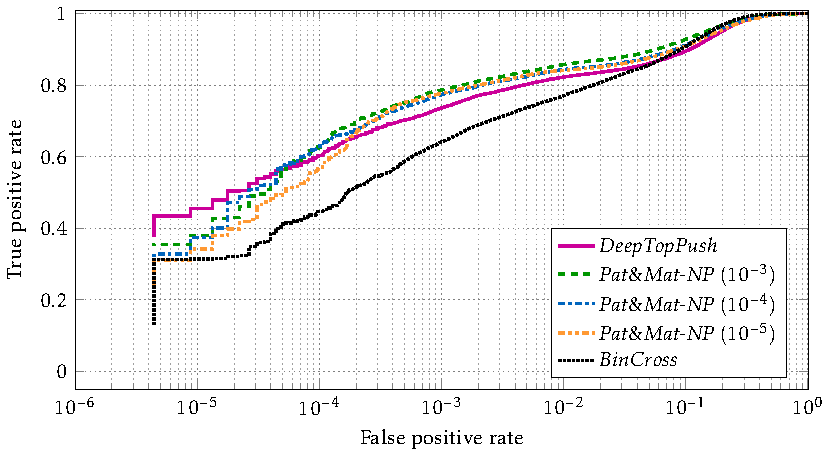
\includegraphics{images/stego_jmipod.pdf}
  \caption{\textbf{JMiPOD dataset:} ROC curves with logaithmic $x$-axis.}
  \label{fig: steganalysis jmipod}
\end{figure}

\begin{table}[!t]
  \centering
  \begin{NiceTabular}{lccccccc}
    \CodeBefore
      \rowcolor{\headercol}{1-2}
      \rowcolors{4}{\rowcol}{}[restart]
    \Body
    \toprule
    \Block[c]{2-1}{\textbf{Formulation}}
      & \Block[c]{2-1}{$\auroc$}
      & \Block[c]{1-3}{$\tpratk$}
      &&& \Block[c]{1-3}{$\tpratfpr$} \\
    \cline{3-8}
      && $1$
      & $10$
      & $5$
      & $10^{-5}$
      & $10^{-4}$
      & $10^{-3}$ \\
    \midrule
    \BaseLine
      & 97.5
      & \worst{13.52}
      & \worst{24.65}
      & \worst{29.54}
      & \worst{27.28}
      & \worst{44.58}
      & \worst{63.84} \\
    \DeepTopPush
      & \worst{97.26}
      & \best{34.25}
      & \best{42.57}
      & \best{47.3}
      & \best{43.59}
      & 60.42
      & 73.67 \\
    \PatMatNP($10^{-5}$)
      & 97.66
      & 21.24
      & 31.6
      & 39.38
      & 33.54
      & 60.35
      & 78.04 \\
    \PatMatNP($10^{-4}$)
      & 97.49
      & 25.66
      & 36.76
      & 45.19
      & 38.28
      & 63.49
      & 77.43 \\
    \PatMatNP($10^{-3}$)
      & \best{98.0}
      & 26.99
      & 38.76
      & 44.83
      & 42.17
      & \best{64.5}
      & \best{78.11} \\
    \bottomrule
  \end{NiceTabular}
  \caption{\textbf{JMiPOD dataset:} All presented results are medians of ten independent runs with different random seeds. Each column of the table corresponds to one performance metric and every row to one formulation. The best result for each metric is highlighted in green, while the worst result is highlighted in red.}
  \label{tab: steganalysis jmipod}
\end{table}

As in the previous subsection, Figure~\ref{fig: steganalysis jmipod} shows ROC curves for the test set of \textbf{JMiPOD} dataset, and Table~\ref{tab: steganalysis jmipod} shows seven performance metrics. Each shown result in this table is a median of ten independent runs. Since trained models use stochastic gradient descent, the results are not as evident as in the case of Nsf5 dataset. \BaseLine still provides the worst results for most of the metrics, but the differences are much smaller than for the Nsf5 dataset. We can see, that \DeepTopPush again provides the best performance for 4 of 7 metrics. It shows that the enhanced minibatch used in \DeepTopPush Algorithm~\ref{alg: deep toppush} improves the approximation quality of the true threshold and therefore it reduces the bias of sampled gradient (as we already showed in Figure~\ref{fig:thresholds2}). Even though \PatMatNP($10^{-3}$), \PatMatNP($10^{-4}$) and \PatMatNP($10^{-5}$) were trained for different levels of false-positive rate, they all perform similarly. As we said before, the decision threshold~$t$ of \PatMatNP model is the approximation of true top $\tau$-quantile of all scores of negative samples. Since we use minibatches with 128 negative samples, the smallest quantile that can be found on this minibatch is~$\tau = \frac{1}{128}=0.0078125.$ If we try to approximate smaller quantiles, we always get the same results. Therefore, \PatMatNP($10^{-3}$), \PatMatNP($10^{-4}$), \PatMatNP($10^{-5}$) should work almost identically, and we can see from both the figure and the table, that these three formulations provide very similar results.

\section{Malware Detection}\label{sec: malware detection}

In the previous section, we presented results from the domain of steganalysis. Another domain in which formulations from presented framework can be very useful, is the domain of malware detection. As an example, consider standard antivirus software on a personal computer. Every user wants to be protected, so the goal of antivirus software is to detect as much malware as possible. However, if the antivirus software is too restrictive, it can easily happen, that clean software is marked as malware, i.e. the antivirus software can easily produce false alarms. If the antivirus software produces false alarms too often, it can be very annoying to the user and may lead to uninstalling the antivirus software. Therefore, the goal of every antivirus software is to maximize a true-positive rate at a very low false-positive rate, which is precisely what the formulations from the framework do.

In this section, we presented results on a real-world dataset provided by a renowned cybersecurity company. The dataset consists of malware analysis reports of executable files. This is an extremely tough dataset as individual samples are JSON files whose size ranges from 1kB to 2.5MB. The structure of the sample is highly complicated because each sample has a different number of features, and features may have a complicated structure, such as a list of ports to which the file connects. This is in sharp contrast with standard datasets, where each sample has the same number of features, and each feature is a real number. The usual approach how to process such complicated data is to create manually feature vectors and use them for training instead of the original data. However, such an approach is extremely time-demanding and requires expert knowledge of the original data. For this reason, we decided to use a different approach that is called Hierarchical Multiple Instance Learning (HMIL)~\cite{pevny2017using}. For the training, we use a publicly available implementation of HMIL~\cite{mandlik2021mill}, which allows train models directly from JSON files without the necessity of complicated feature extraction.

Since the dataset is very large (see Table~\ref{tab: datasets summary}), we train each formulation only one time. Moreover, we use only the formulations that worked the best in the previous experiments, i.e. we use only the \BaseLine, \PatMatNP($10^{-2}$), \PatMatNP($10^{-3}$) and \BaseLine. As an optimizer, we use the ADAM~\cite{kingma2014adam} with default settings and fixed step length~$\alpha = 0.01.$ We also use balanced mini-batches of size 2000, which allows us to obtain a very good estimate of the true thresholds as discussed in Section~\ref{sec: biased threshold estimate}. Finally, we use a fixed number of epochs to 100 for all formulations.

Figure~\ref{fig: malware detection} shows the performance of all formulations on the test set. For the comparison, we use ROC curves and we use filled circles to highlight the thresholds for which the formulation were optimized. It is clear, that \DeepTopPush is the best at low false-positive rates. Even at the extremely low false positive rate $\tau=10^{-5}$, \DeepTopPush correctly identified $46\%$ of malware. We can also see, that \PatMatNP($10^{-3}$) is the best at false-positive rate~$10^{-3}$, which is exactly the point for which the formulation should be optimized. However, \DeepTopPush performs almost as well as \PatMatNP($10^{-3}$) at this false-positive rate. Finally, at the false-positive rate~$10^{-2}$ all formulations perform equally well.

\begin{figure}
  \centering
  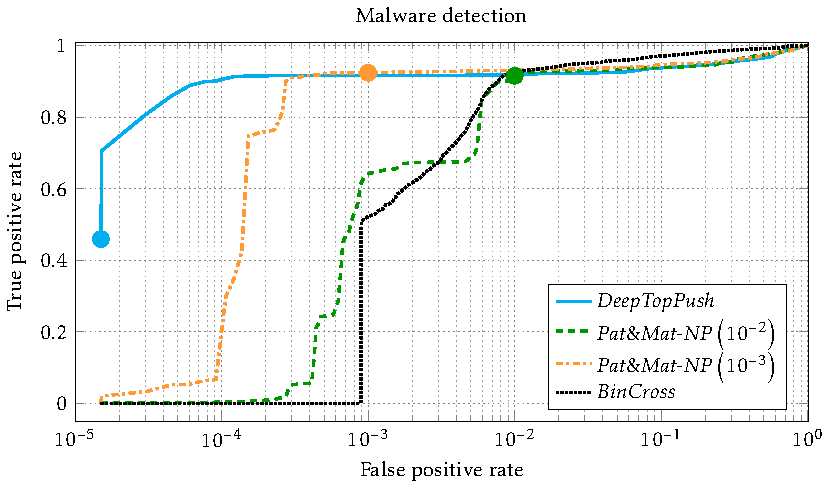
\includegraphics{images/malware_detection.pdf}
  \caption{\textbf{Malware detection:} ROC curves with logaithmic $x$-axis. The circles show the thresholds the formulations were optimized for.}
  \label{fig: malware detection}
\end{figure}
